% ################################################################### Complexity1
\chapter{Результаты}
\section{Разработка и верификация метода оценки изменчивости генома на основе графового представления расположения генов} \label{chaptComplex1}

\subsection{Разработка способа представления расположения генов в виде графа}
Рассмотрим три условные генома, показанные в верхней части рисунка~\ref{img:graph_scheme}. Предположим, что мы установили группы гомологии и стрелками одного цвета показаны гомологичные гены. Для представления этого набора геномов в виде графа, будем ставить в соответствие каждому множеству гомологичных генов узел графа. Ребрами соединим узлы, для которых гены из соответствующих групп гомологии расположены последовательно хотя бы в одном геноме. Вес ребра установим в количество геномов, подтверждающих данную связь (в этих геномах соответствующие гены расположены последовательно). Таким образом мы закодировали информацию о расположении генов в наборе геномов в виде графа (нижняя часть рисунка~\ref{img:graph_scheme}). 

В рассмотренном примере, мы представили  три генома, содержащих суммарно 21 ген, в виде графа из 10 узлов. Чем большее количество геномов будет использовано в анализе, тем выше будет "экономия"\ --- разница между количеством генов и количеством узлов в построенном графе.

\begin{figure}[!ht] 
  \center
    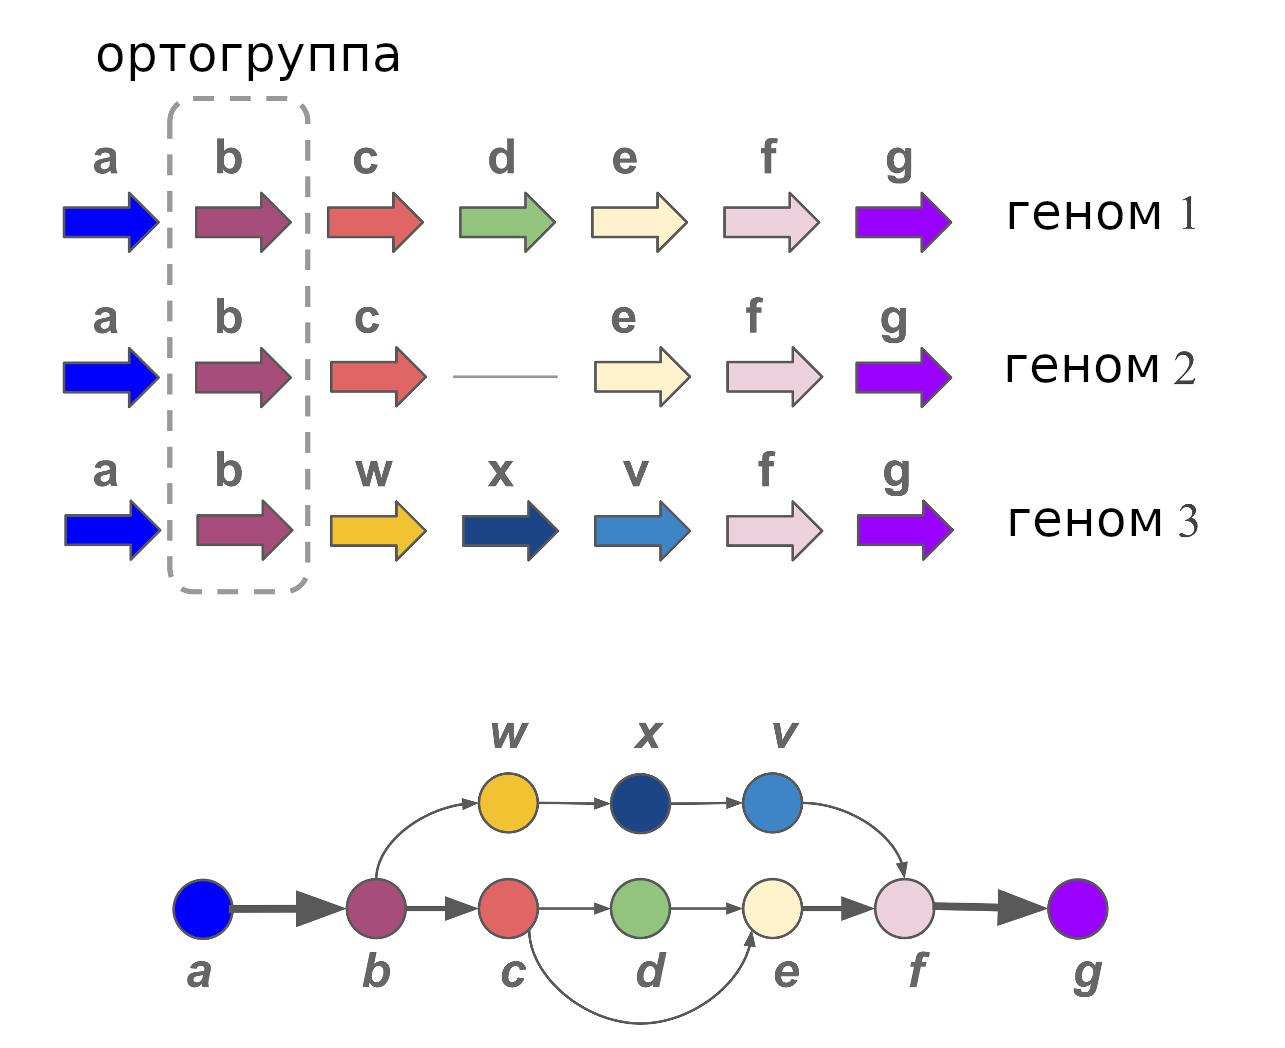
\includegraphics [width=0.9\textwidth] {Dissertation/images/graph/graph_scheme.png}
    \caption{Представление контекста генов в виде графа. Рассматриваем три гипотетеических генома, состоящих из 6-7 генов. Гены показаны стрелками, цветом и буквами обозначены гены, относящиеся к одной ортогруппе. В нижней части рисунка показано графовое представление для данного набора геномов.}
    \label{img:graph_scheme}
\end{figure}

Мы выбрали способ представления  набора геномов в виде направленного графа:  ребра имеют направление, соответствующие обходу генома от начала к концу. Это было сделано для того, чтобы сохранить всю информацию о порядке расположения генов, в частности о геномных инверсиях. Рассматриваемые геномы при этом должны быть ориентированы единообразно. В публичных базах геномов (RefSeq, GenBank, Patric и другие) не предусмотрено требований к ориентации последовательностей: они начинаются с произвольных позиций и могут быть ориентированы в произвольном направлении. Поэтому перед построением графа, мы производим согласование ориентаций геномов друг с другом. Для этого выбирается референсный геном (произвольно, из финишированных геномов), затем для каждого генома устанавливаются области синтении (относительно референсного генома); подсчитывается сумма произведений длин блоков на нуклеотидное сходство для всех блоков в прямой и обратной ориентации; в зависимости от того, какая из сумм оказалась выше, оставляется либо исходная ориентация, либо она меняется на противоположную. Если рассматриваемый геном состоит из нескольких контигов, то согласование ориентации с референсом производится для каждого контига в отдельности.

Скрипт на языке R, выполняющий согласование ориентаций генома и построение графа доступен по адресу \url{https://github.com/paraslonic/graph_complexity/scripts/OG2graph.r}. На вход ему подается таблица групп гомологии в формате выдачи программы OrthoFinder - текстовый файл, каждая строка которого соответствует одной группе гомологии и имеет формат: <идентификатор группы>: <ген1> <ген2> ... <ген n>. На выходе создается файл paths.sif, содержащий граф в формате sif: <идентификатор группы 1> <идентификатор группы 2> <геном>. 

Для автоматизации представления набора геномов в виде графа мы реализовали вычислительный конвейер, схема которого представлена на рисунке~\ref{img:graph_pipe_schema}. В нем осуществляются следующие шаги: 1) аннотация геномов (выделение белок-кодирующих областей), 2) форматирование файла в формате FASTA с аминокислотными последовательностями генов (в заголовках последовательностей мы указываем информацию о расположении генов), 3) построение групп гомологий и 4) формирование графа. На вход подается набор нуклеотидных последовательностей геномов в формате FASTA, выходом является граф в формате sif. Данный конвейер реализован в системе управления рабочим процессом snakemake и доступен по адресу \url{https://github.com/paraslonic/graph_complexity}.

\begin{figure}[!ht] 
  \center
    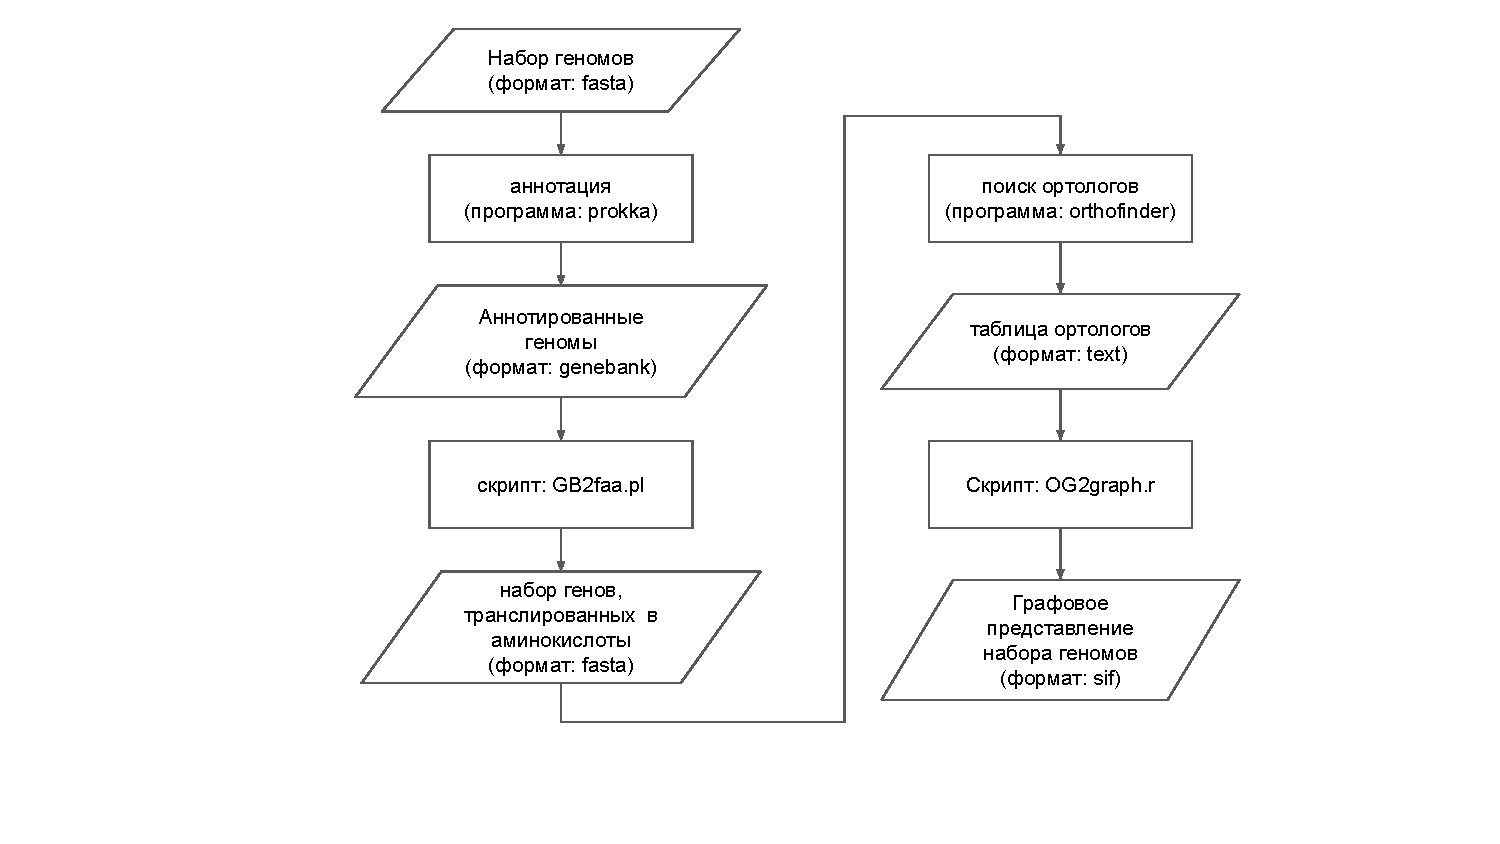
\includegraphics [width=\textwidth] {Dissertation/images/graph/graph_complexity_schema.pdf}
    \caption{Вычислительный конвейер для представления контекста генов в наборе геномов в виде графа.}
    \label{img:graph_pipe_schema}
\end{figure}

\subsection{Разработка алгоритма оценки изменчивости генома на основе графового представления}

Предположим, что в ходе эволюции, в рассматриваемой группе геномов, наблюдались лишь изменения микро-масштаба -- однонуклеотидные замены. В таком случае, набор и взаимное расположение генов не изменялись и соответствующий граф будет содержать лишь один путь. Любые изменения в составе, либо расположении, генов (делеции, вставки, перемещения) будут приводить к появлению новых ребер и новых узлов (в случае вставки нового гена). Чем больше узлов и ребер содержит граф --- тем больше возможных путей его обхода. Это позволяет использовать количество путей в графе в качестве меры вариабельности генома.

Разные фрагменты генома могут существенно различаться по уровню изменчивости. Ниже мы опишем процедуру построения профиля изменчивости генома. Данный профиль отражает как уровень изменчивости меняется вдоль хромосомы (либо иного репликона). Для подсчета уровня локальной изменчивости в отдельном фрагменте генома происходит подсчет количества путей в подмножестве графа (подграфе), соответствующему данному фрагменту. Локальная изменчивость подсчитывается во всех возможных локусах генома и таким образом получается профиль изменчивости. Иначе говоря, мы проходим по геному скользящим окном, выбирая области фиксированного размера (ширина окна задается пользователем) и оцениваем количество зафиксированных изменений в этих областях.

Принцип подсчета локальной вариабельности генома проиллюстрирован на рисунке~\ref{img:complexity_scheme}. Из множества геномов выбирается один геном, служащий референсом (для него будет производиться построение профиля вариабельности). Путь, соответствующий чередованию генов в референсном геноме будем называть базовым путем (узлы этого пути обозначены зеленым цветом). Рассмотрим некоторую окрестность гена Х, ограниченную тремя генами слева и справа от гена Х. Произведем поиск путей, которые начинаются (исходят из базового пути) и заканчиваются (возвращаются в базовый путь) внутри рассматриваемой окрестности и при этом не проходят через узел Х --- такие пути будем называть обходными путями. Суммарное количество обходных путей принимается в качестве меры локальной вариабельности генома окрестности гена Х. На нижней части рисунка~\ref{img:complexity_scheme} показаны примеры: слева --- участка с низкой вариабельностью и двумя обходными путями, справа --- с более высокой вариабельностью и шестью обходными путями. Для получения профиля вариабельности, мы рассчитываем локальную вариабельность для каждого гена из референсного генома.  

\begin{figure}[!ht] 
  \center
    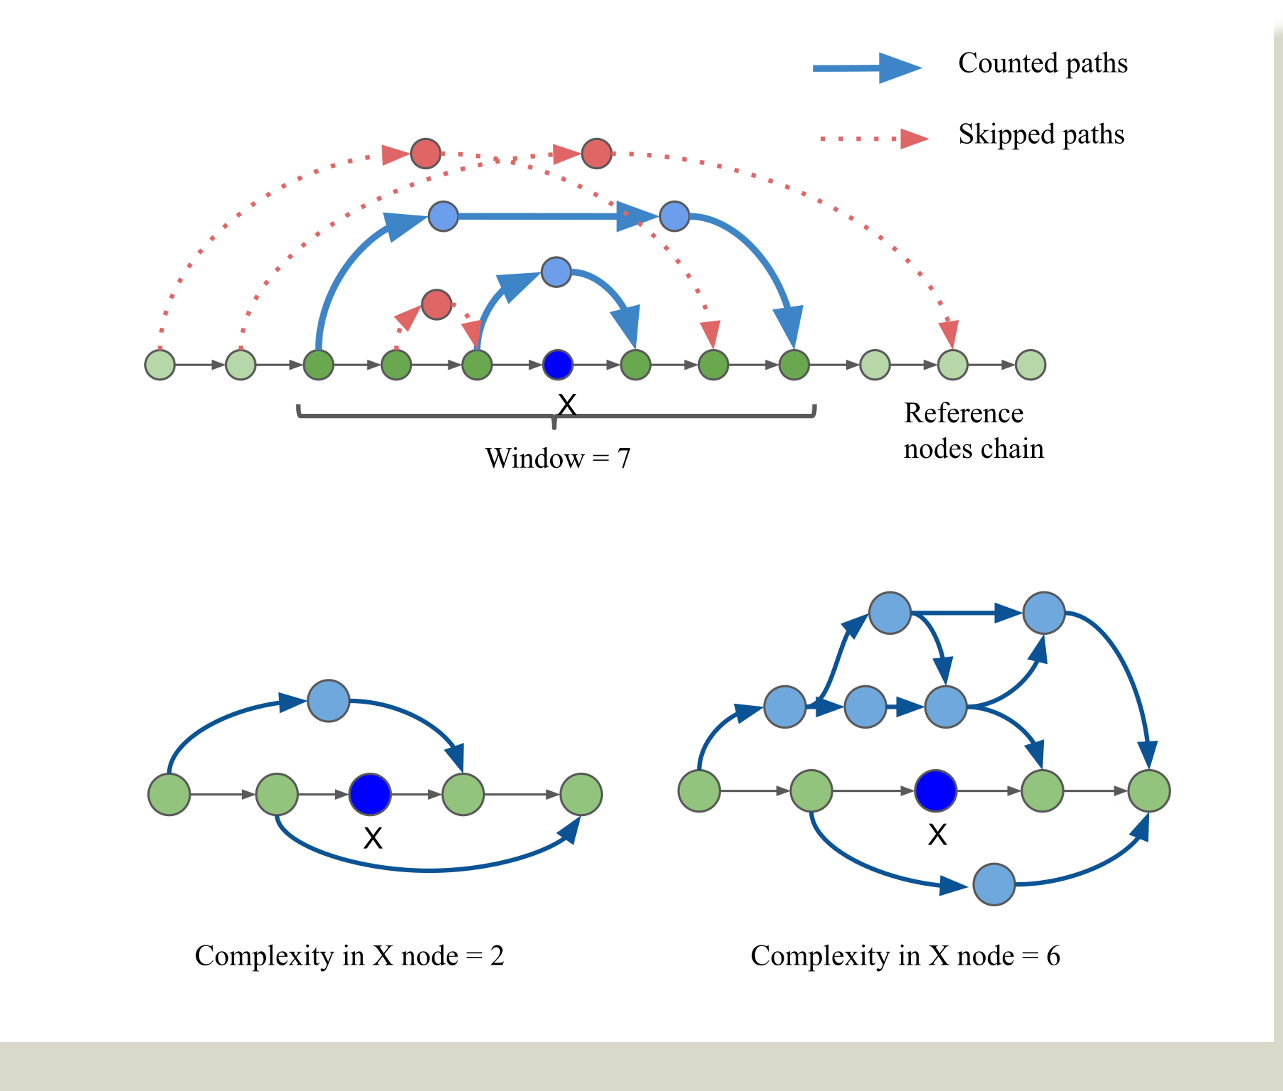
\includegraphics[width=0.8\textwidth]{Dissertation/images/complexity_scheme.png}
  \caption{Подсчет локальной вариабельности генома на основе количества путей в графе. Вверху показан подграф, представляющий окрестность гена X. Ребра черного цвета являются частью базового пути, который соответствует порядку генов в референсном геноме, ребра синего цвета --- обходным путям, а ребра красного цвета --- путям, которые не вносят вклад в значение вариабельности. На нижней части рисунка приведен пример графа с низкой (слева) и высокой (справа) вариабельностью, указаны соответствующие количества обходных путей.}
  \label{img:complexity_scheme} 
\end{figure}



%###########################################################################################

\subsection{Верификация предложенного метода оценки профиля изменчивости генома}
Мы провели верификацию предложенного подхода оценки профиля изменчивости и его программной реализации при помощи: 1) симуляции эволюции геномов; 2) сравнения результатов нашего метода с ранее опубликованными оценками других авторов. 

\subsubsection{Симуляция эволюции геномов}
Мы проводили моделирование эволюции геномов на основе задаваемого профиля изменчивости. Данный профиль определял вероятности изменений генного состава в зависимости от положения гена в геноме. Мы использовали следующие варианты изменений: вставки либо удаления генов, перемещения генов, инверсии фрагментов моделируемого генома. Мы использовали несколько профилей изменчивости, для каждого из которых проводили моделирование геномных изменений, оценивали профиль изменчивости предложенным нами методом и сравнивали полученный результат с изначально заданным профилем. Нашей целью была проверка применимости предложенного метода в том случае, когда в геноме присутствуют области пониженной и повышенной изменчивости.

Модельный геном представлял из себя последовательность целых чисел (n=5000). Вначале, создавались одинаковые геномы. Далее, проводилось 3000 итераций, в каждой из которых происходило изменение генома. Локализация изменений определялась на основе профиля изменчивости. Вероятности вставки и удаления генов были выбраны равными друг другу (для сохранения длины геномов), вероятности геномных инверсий были в 100 раз меньше (оценка получена исходя из литературных данных). Длины инверсий, вставок и делеций выбиралась случайно, на основе экспоненциального распределения (изменения малой длины были более вероятны, чем изменения большой длины). Вставка генов производилась из набора, размер которого в два раза превышал исходный набор генов (исходно в геноме были числа от 0 до 5000, вставлялись числа от 5000 до 15000).

Профили изменчивости были следующих типов: 1) ступенчатый, 2) синусоидальный, 3) пилообразный. Для каждого профиля изменчивости проводилось 10 симуляций. На рисунке~\ref{img:simulation} приведен пример сравнений исходного профиля изменчивости (слева) и профиля, полученного в результате анализа предложенным нами способом (справа). В таблице \ref{simulation_table} приведены средние значения R$^{2}$ и коэффициента корреляции исходного профиля изменчивости и профиля, полученного в результате анализа и усредненного по 10 повторам. 

\begin{figure}[!ht] 
  \center
    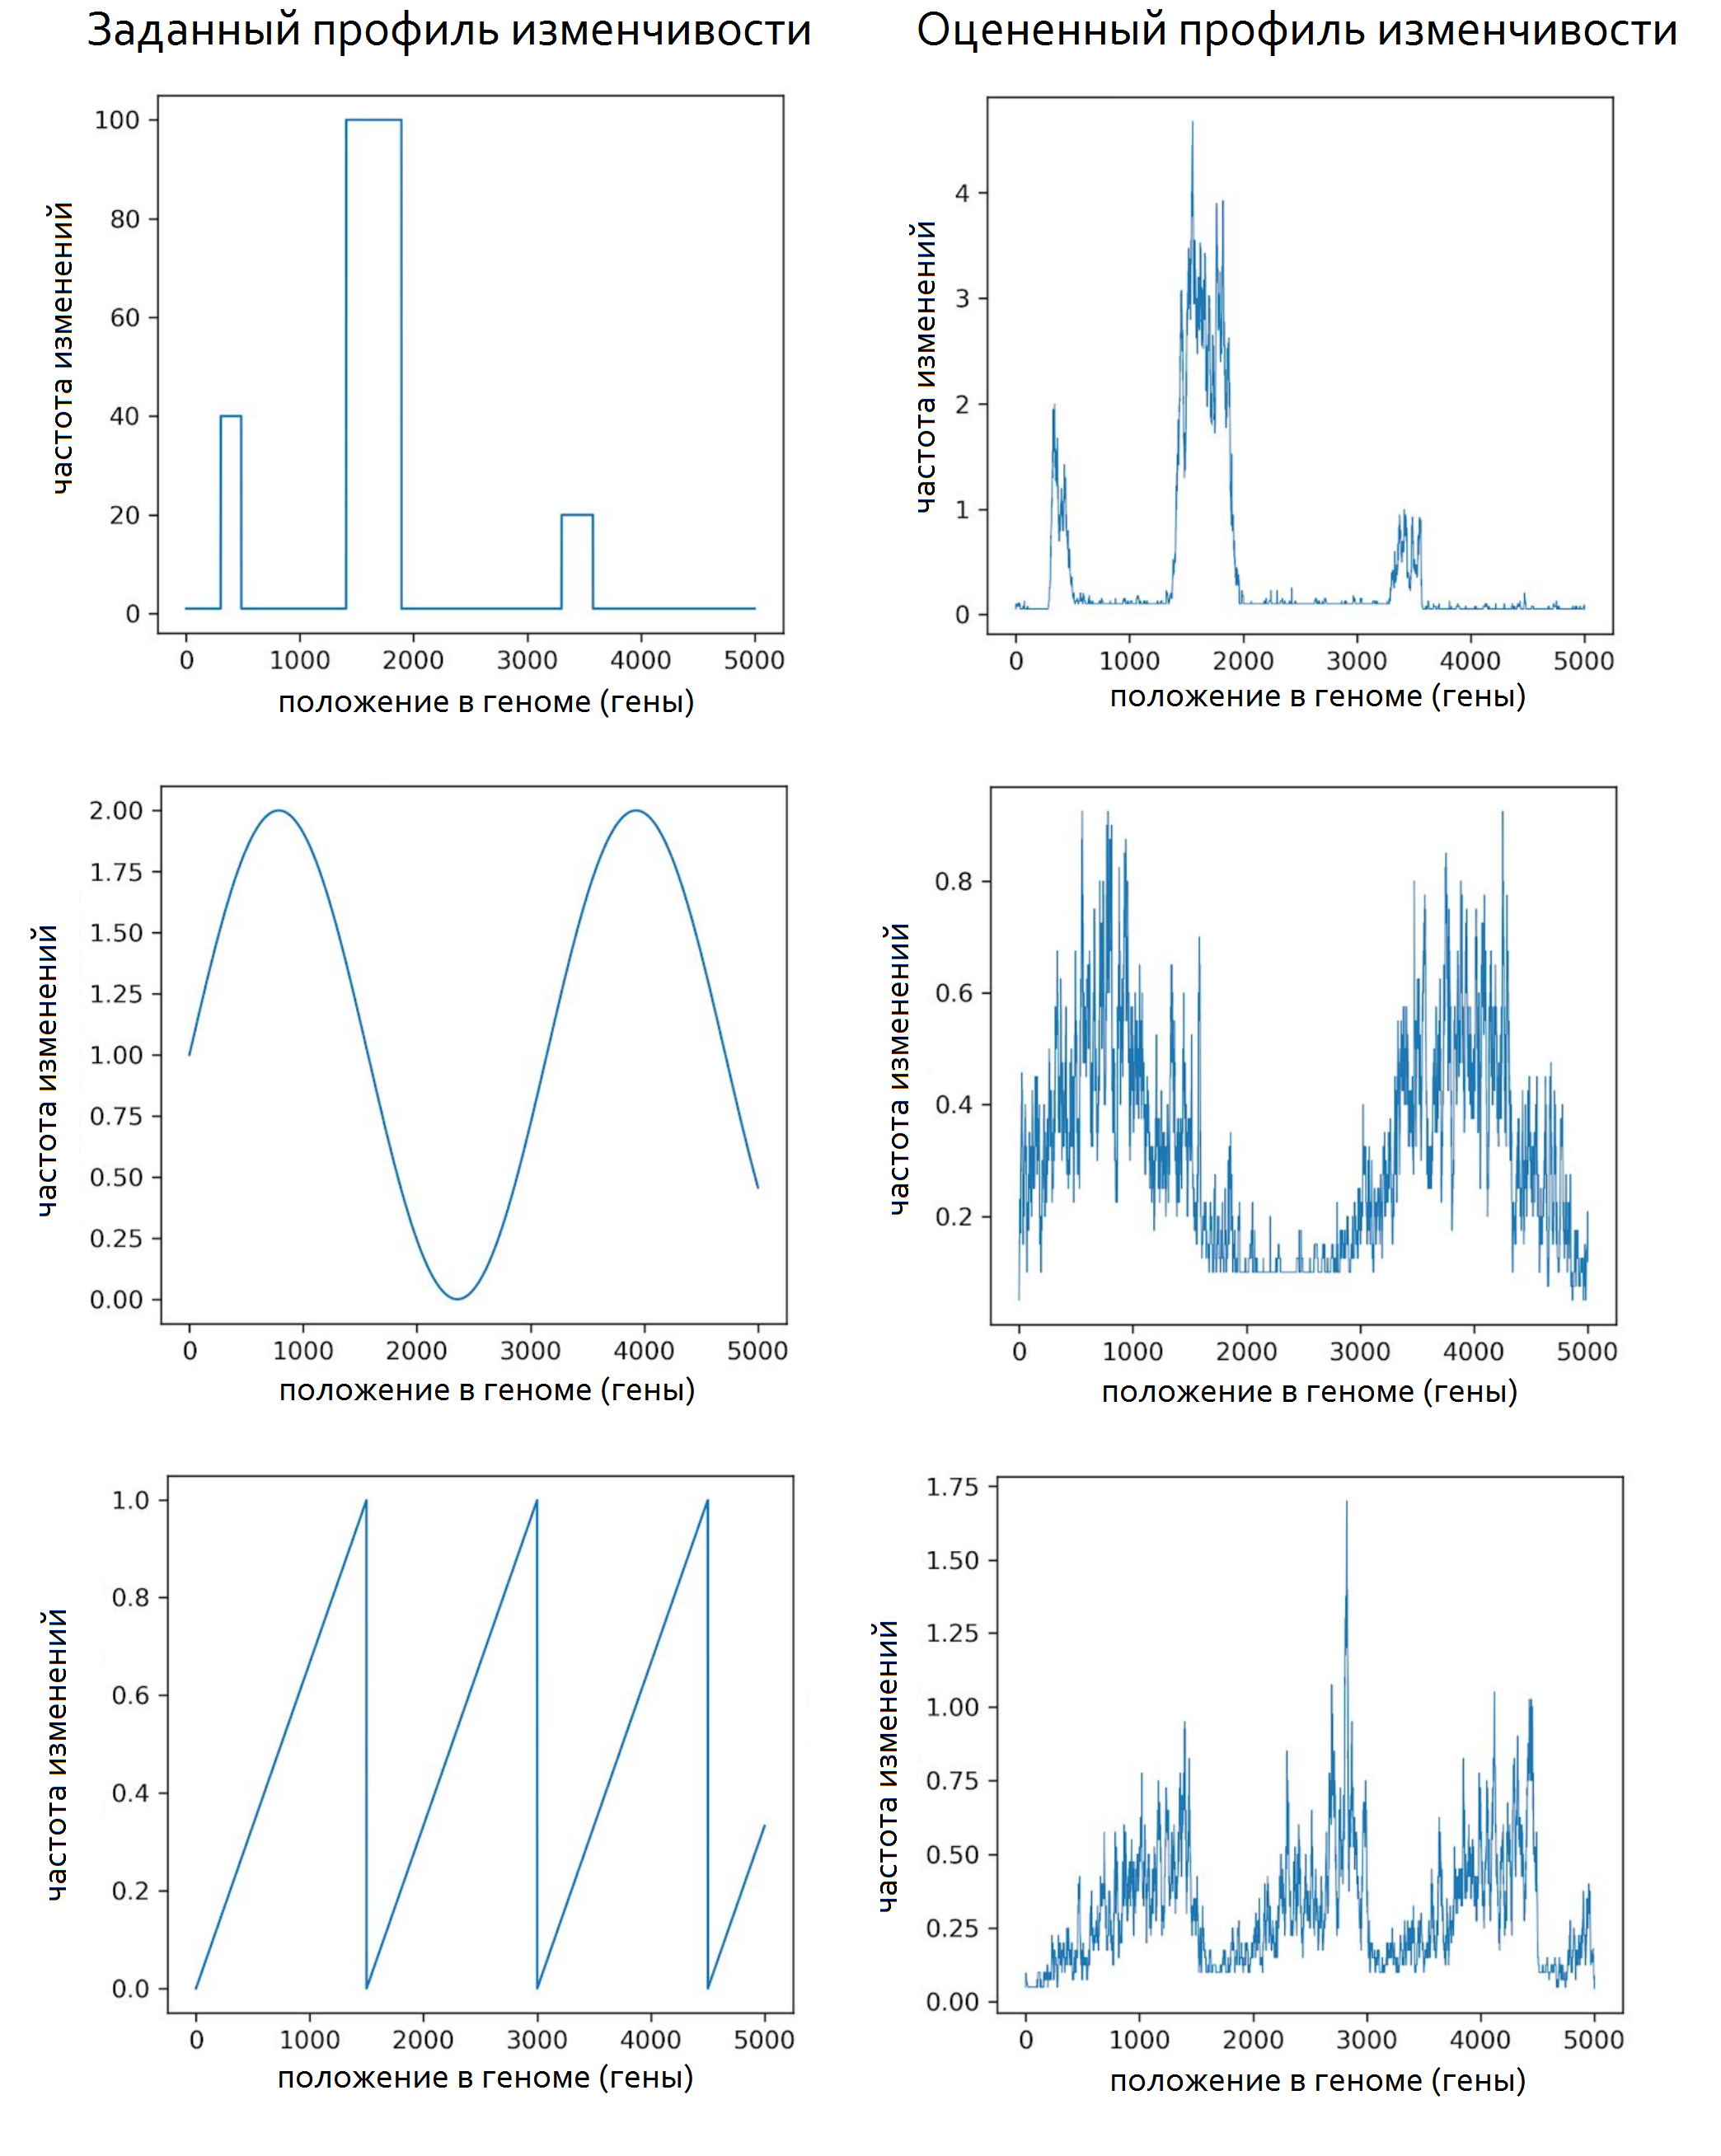
\includegraphics[width=0.8\textwidth]{Dissertation/images/complexity/simulation.png}
  \caption{Сравнение профиля изменчивости, задаваемого для моделирования геномных изменений (слева), и профиля, получаемого в результате анализа предложенным нами методом (справа). }
  \label{img:simulation} 
\end{figure}

\begin{table} [htbp]
  \centering
  \parbox{15cm}{%
      \caption{Результаты сравнения задаваемого при моделировании и оцененного профиля изменчивости при разной форме профиля.}\label{simulation_table}%
  }
\begin{tabular}{ | l | l | l | }
\hline
Тип профиля & Значение R$^{2}$ & Коэффициент корреляции Спирмена\\ \hline
Ступенчатый & 0.95 & 0.69 \\ \hline
Синусоидальный & 0.77 & 0.82 \\ \hline
Пилообразный & 0.80 & 0.85 \\ 
\hline
\end{tabular}
\end{table}

Отметим, что значительное влияние на точность оценки профиля изменчивости оказывает частота геномных инверсий: чем она выше - тем была ниже точность. Таким образом, частые перестройки генома служат существенным ограничением применимости предложенного метода. 

\subsubsection{Сравнения результатов предложенного метода с ранее опубликованными оценками других авторов}
В работе \cite{oliveira2017chromosomal} авторы проводили поиск горячих точек горизонтального переноса генов (ГПГ) для 80 бактериальных видов. Мы провели сравнение найденных ими горячих точек с профилем изменчивости генома, оцененным описанным выше способом. На рисунке~\ref{img:rocha_comparison} приведен пример сравнения результатов двух методов для генома \textit{E. coli}. Видно, что, в данном случае, оба метода хорошо согласуются между собой.     

\begin{figure}[!ht] 
  \center
    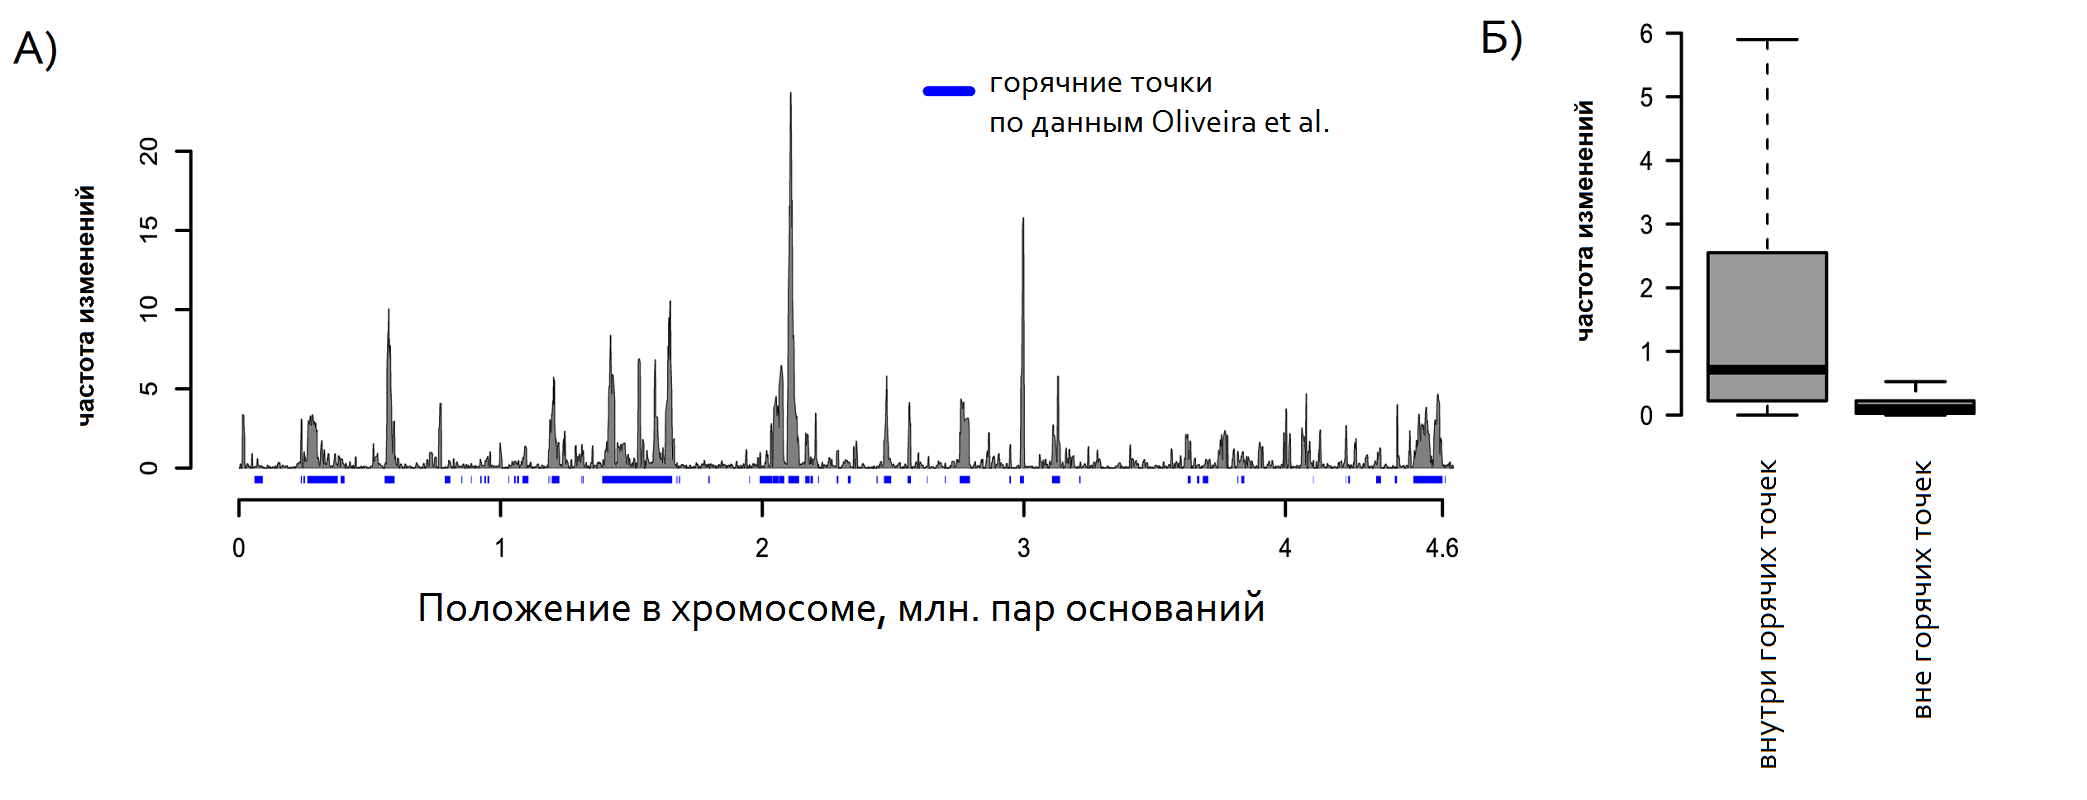
\includegraphics[width=\textwidth]{Dissertation/images/complexity/rocha_comparepng.png}
  \caption{Сравнение профиля изменчивости \textit{E. coli K12 MG1655}, установленного нашим методом, с областями повышенной изменчивости (``горячими'' точками горизонтального переноса) генов в работе Oliveira et al. \cite{oliveira2017chromosomal}. }
  \label{img:rocha_comparison} 
\end{figure}

Для других видов бактерий, мы наблюдали как хорошо согласующиеся между собой, так и весьма непохожие результаты (например, в случае \textit{Brucella melitensis} и \textit{Burkholderia pseudomallei}). Расхождение может быть следствием: 1) малого количества геномов используемого для анализа в работе \cite{oliveira2017chromosomal} (для многих видов оно было меньше 20, в среднем 12 геномов для одного вида), что значительно ухудшает соотношение сигнал/шум как нашего, так вероятно и используемого в работе \cite{oliveira2017chromosomal} метода, 2) различием в подходах для оценки изменчивости (мы берем в рассмотрения все события, затрагивающие изменение порядка генов, не только горизонтальный перенос генов). Выяснение точной причины расхождений затруднено, поскольку авторами работы \cite{oliveira2017chromosomal} не предоставляется программная реализация метода.

%###########################################################################################
\section{Исследование применимости метода оценки локальной вариабельности генома}

\subsection{Зависимость результатов от размера выборки}

Чем больше геномов будет использовано для анализа, тем полнее будет получено представление о возможных вариантах со-расположения генов. Слишком маленькое количество геномов приведет к понижению чувствительности анализа и снизит соотношение сигнал/шум. В тоже время, слишком большое количество геномов потребует значительных вычислительных ресурсов и приведет к увеличению времени анализа. Поэтому, актуален вопрос о зависимости результатов анализа от размера выборки и определение минимально допустимого количества геномов.

На рисунке~\ref{img:genome_number} показан график зависимости коэффициента корреляции профиля вариабельности, рассчитанного на основании 100 геномов, либо на основании выборки меньшего размера. Для анализа использованы финишированные геномы \textit{E. coli}. Для каждого размера выборки геномов проводилось 10 испытаний, для чего геномы выбирались случайным образом из полного набора. 

\begin{figure}[!ht] 
  \center
    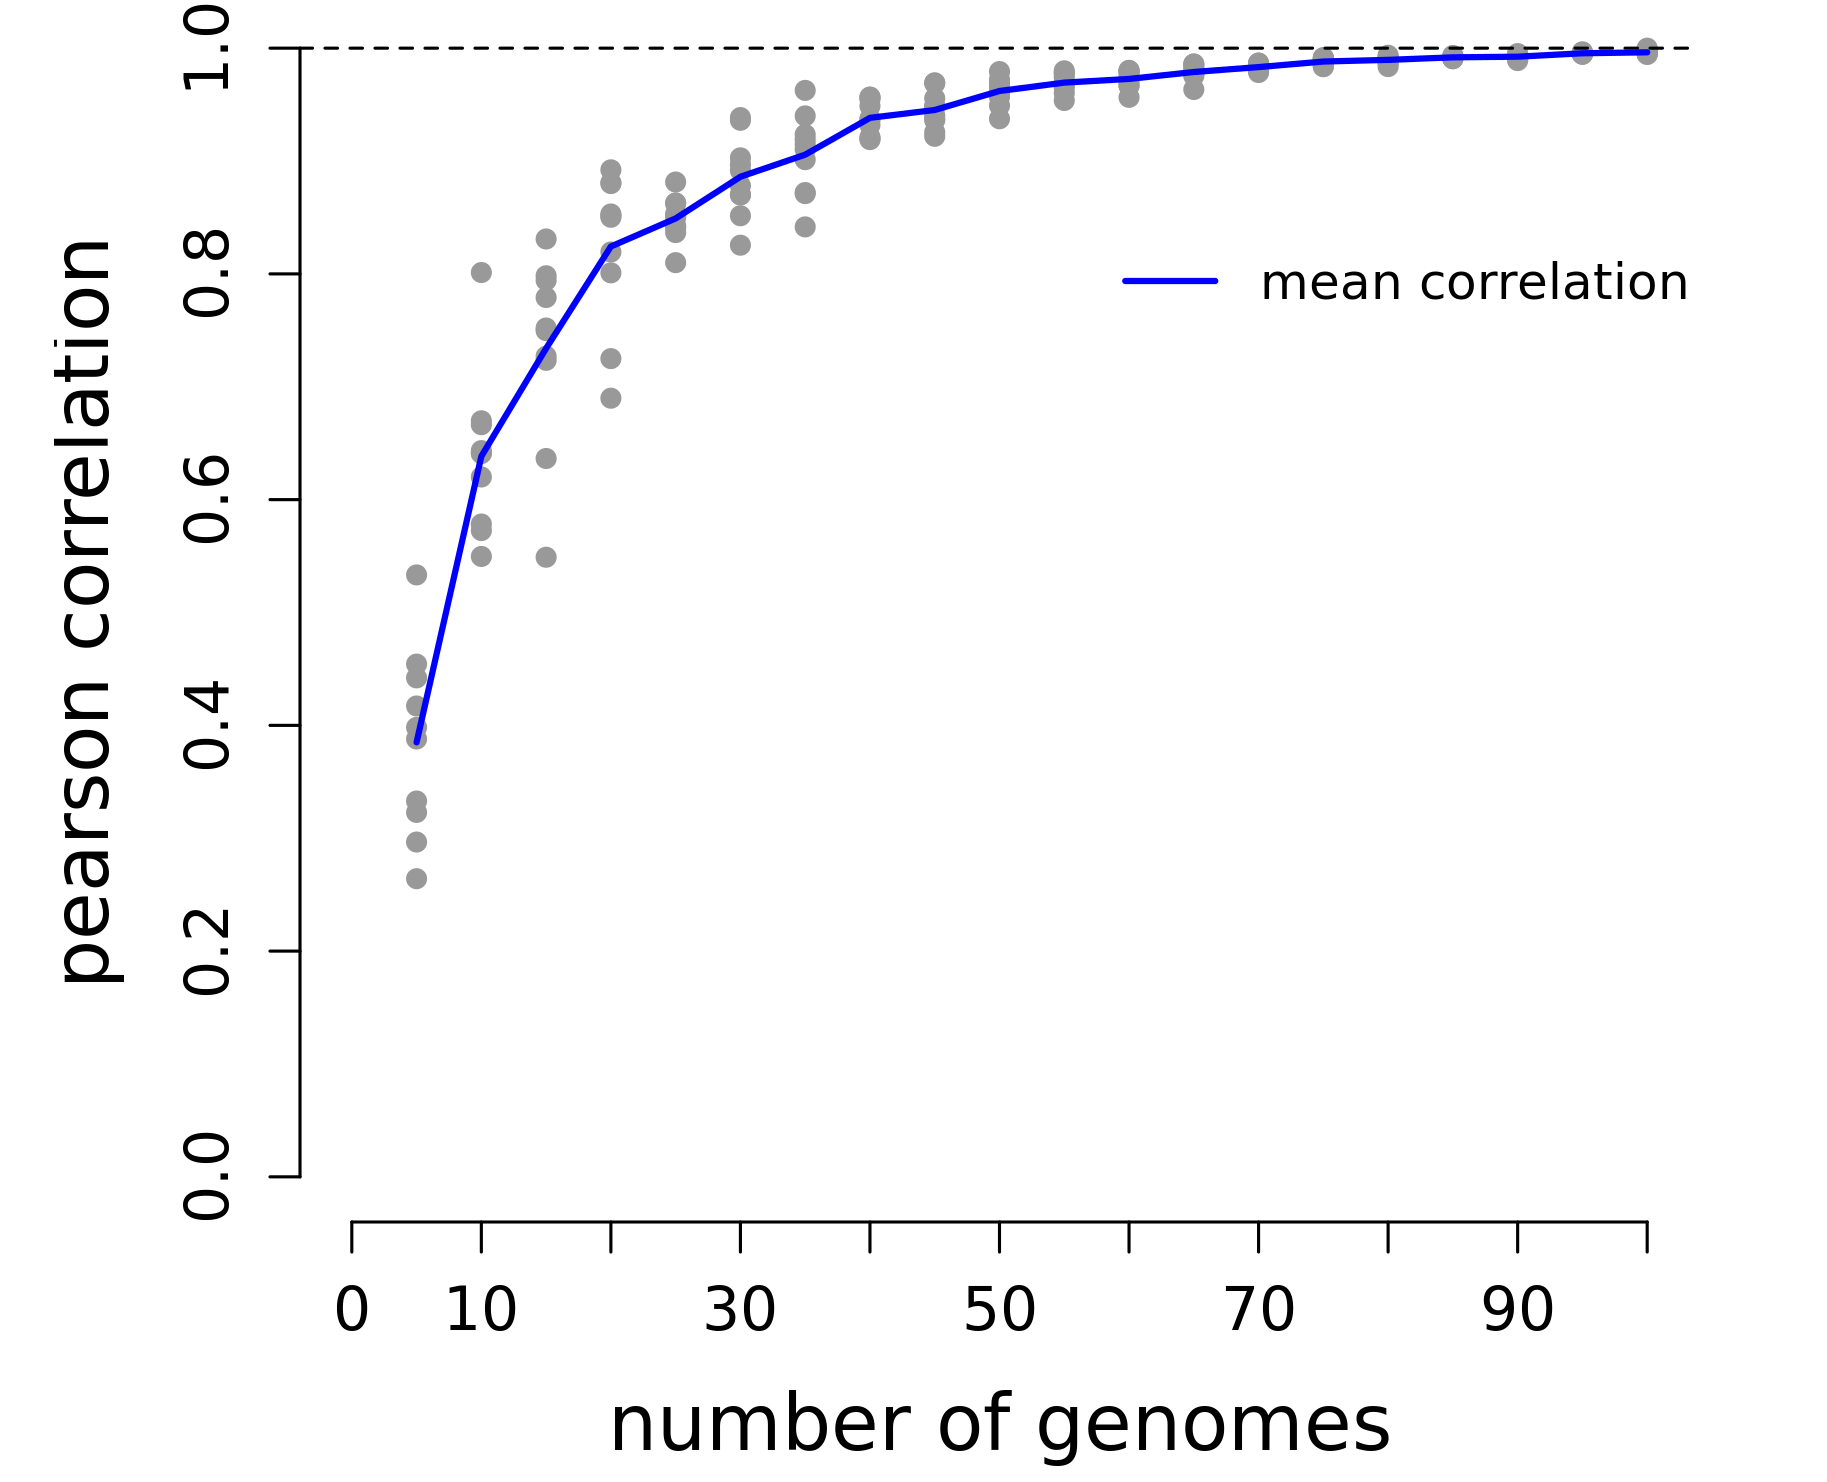
\includegraphics[width=0.5\textwidth]{Dissertation/images/complexity/numberOfGenomes.png}
  \caption{Значение коэффициента корреляции профиля вариабельности, оцененной на основе 100 геномов с профилями оцененными на основе меньшего количества геномов. Синяя линия проведена по значениям корреляции, усредненным по 10 испытаниям. }
  \label{img:genome_number} 
\end{figure}

При количестве геномов большем чем 50, значение коэффициента корреляции превышало уровень 0.9. В дальнейшем, мы ориентировались на эту оценку и брали в рассмотрение лишь те виды, для которых доступное количество геномов составляло не менее 50.

На рисунке~\ref{img:complex_runtime} показана зависимость времени, необходимого для построения графа и анализа профиля вариабельности от количества геномов. Анализ проводился на основании финишированных геномов \textit{E. coli}. Видно, что зависимость носит линейный характер. Анализ проводился в один поток на персональном компьютере с процессором i7 9750h. Наиболее продолжительным шагом общего анализа является этап построения групп гомологии. Так, для тысячи геномов, время анализа составило пять суток, анализ проводился в 50 потоков на вычислительном кластере на основе процессоров AMD EPYC 7502.

\begin{figure}[!ht] 
  \center
    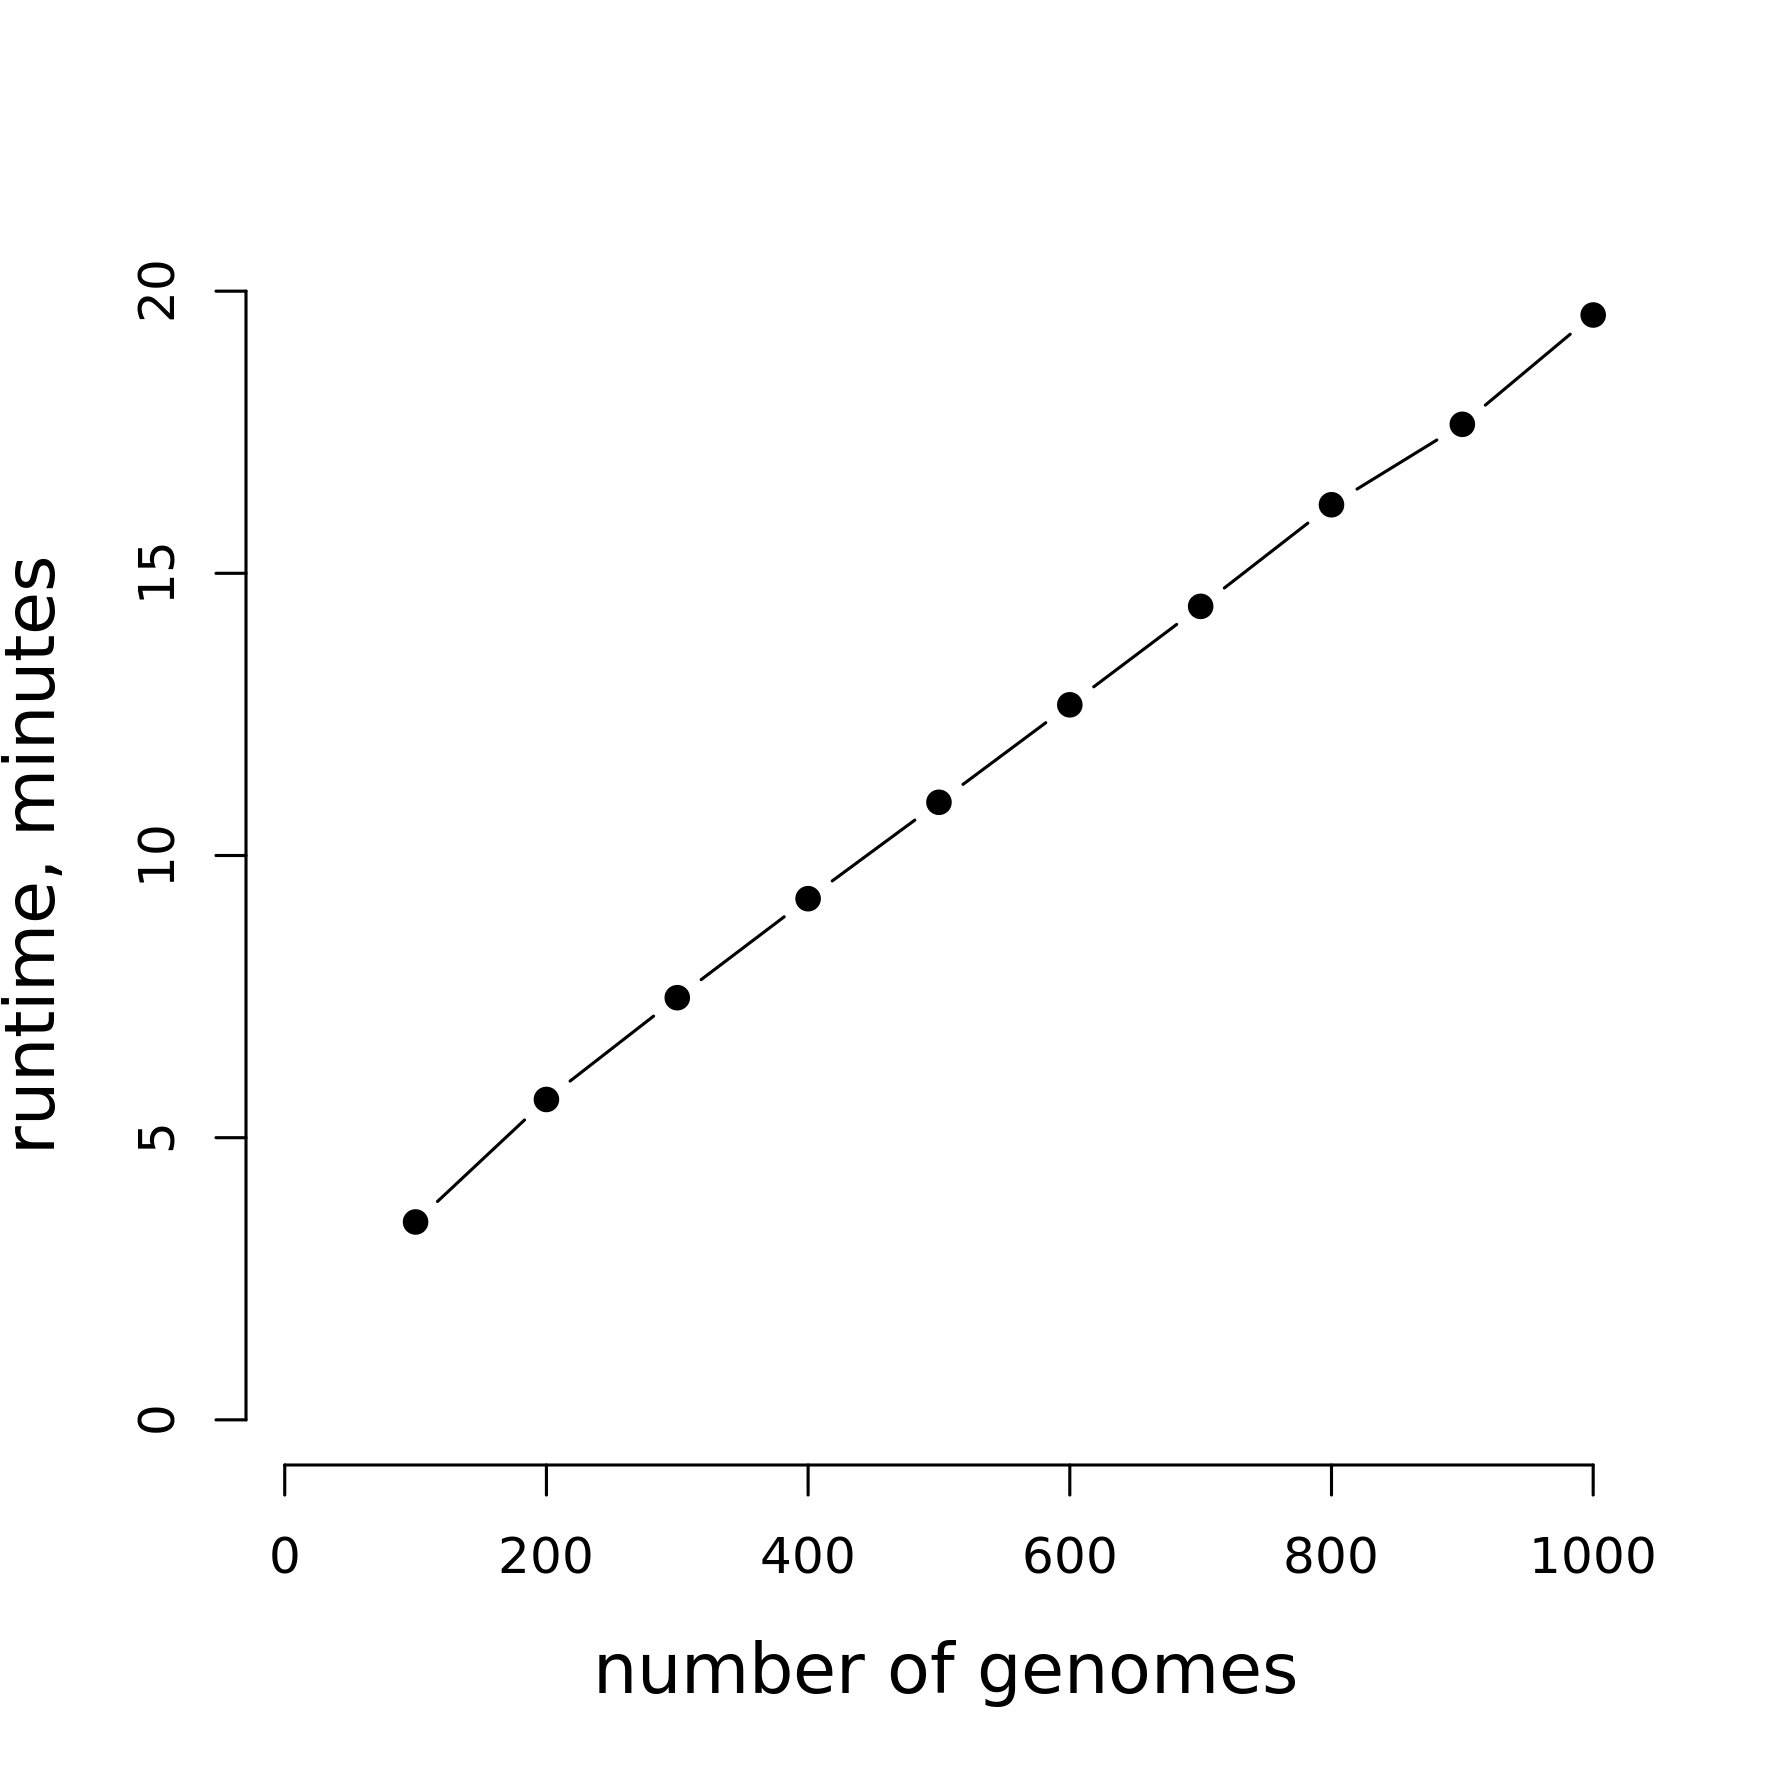
\includegraphics[width=0.8\textwidth]{Dissertation/images/complexity/runtime_nocoalign.png}
  \caption{Зависимость времени, необходимого для построения графа и расчета профиля изменчивости, от количества геномов. Для анализа использованы финишированные геномы \textit{E. coli}. }
  \label{img:complex_runtime} 
\end{figure}

\subsection{Анализ зависимости результатов от качества сборки генома}

Многие геномы прокариот собраны не до уровня репликонов, но состоят из контигов - фрагментов генома, которые удается собрать из коротких прочтений, без применения дополнительных экспериментальных методов. 
Для анализа чувствительности алгоритма к типу входных данных: финишированные (собранные до уровня репликонов), либо фрагментированные геномы (состоят из контигов), мы выбирали случайным образом по 100 геномов одного либо другого типа и оценивали профили вариабельности по одному и тому же референсному геному. Сравнение профилей по финишированным либо фрагментированным геномам для двух видов бактерий показано на рисунке~\ref{img:compl_dr_coli}. Видно, что профили обладают значительной степенью сходства (коэффициент корреляции Пирсона составил 0.87 и 0.81 для \textit{E. coli} и \textit{Pseudomonas aeruginosa}, соответственно). 

\begin{figure}[!ht] 
  \center
    \subcaptionbox{}{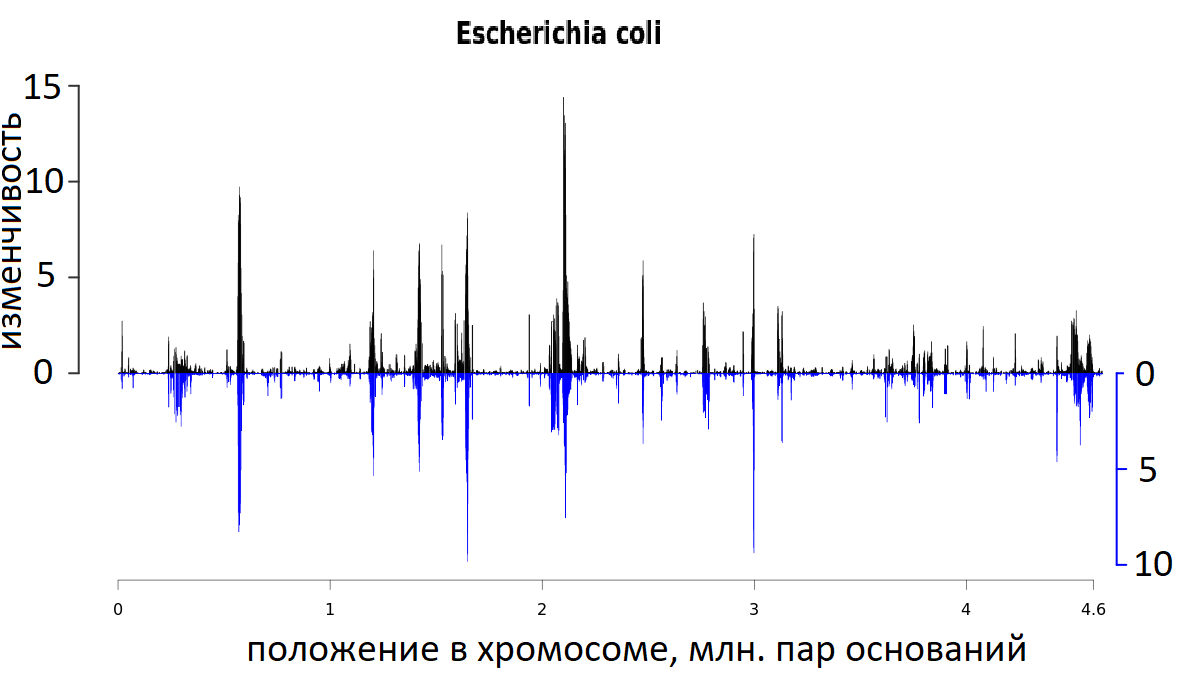
\includegraphics[width=0.8\textwidth]{Dissertation/images/complexity/complete_draft_coli.png}}
    \subcaptionbox{}{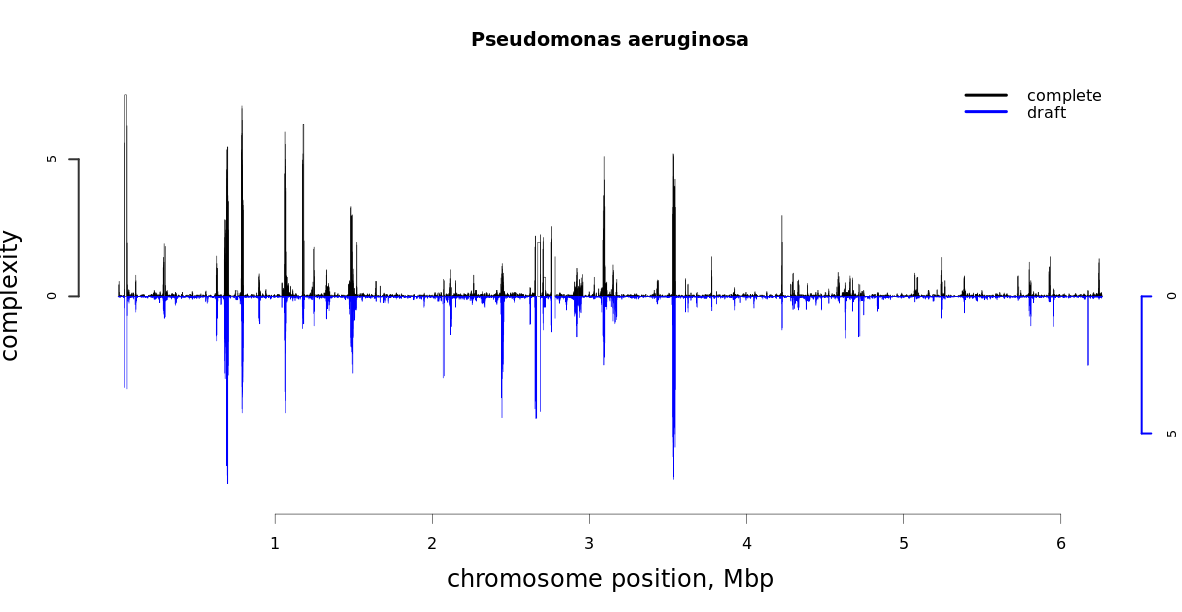
\includegraphics[width=0.8\textwidth]{Dissertation/images/complexity/complete_draft_paeru.png}}
  \caption{Сравнение профилей вариабельности 100 финишированных и 100 фрагментарных геномов видов: а) \textit{E. coli}, б) \textit{Pseudomonas aeruginosa}. Черным цветом показан профиль вариабельности на основе финишированных геномов, синим - на основе собранных до уровня контигов.}
  \label{img:compl_dr_coli} 
\end{figure}

Заметим, что значения профиля изменчивости зависят от набора геномов, используемых для сравнения. Мы выбирали случайные геномы в наборы финишированных и фрагментированных геномов, что также вносило вклад в наблюдаемое различия профилей. Вклад собственно качества сборки геномов еще меньше наблюдаемого выше уровня различий. Основываясь на этой оценке, мы считали, что финишированность геномов не является обязательным для включения геномов в анализ.

%№№№№№№№№№№№№№№№№№№№№№№№№№№№№№№№№№№№№№№№№№№№№№№№№№№№№№№№№№№№№№№№№№№№
\section{Применение метода оценки локальной вариабельности генома}


\subsection{Профиль вариабельности генома \textit{E. coli}}
На рисунке~\ref{img:complexity_lf82} показан профиль изменчивости генома \textit{E. coli LF82}, рассчитанный на основании графового представления 326 геномов других штаммов данного вида. Цветом обозначены жизненно-необходимые гены (мутации в которых летальны), гены транспортных и рибосомных РНК, острова патогенности и места встройки профагов, описанные для данного генома. Видно, что большая часть локусов с повышенной вариабельностью ("горячие точки"\ изменчивости) находятся именно в тех местах, где у данного штамма находятся профаги, либо острова патогенности. Гены транспортных и рибосомных РНК не имеют очевидной связи с профилем вариабельности. 

Отметим, что фрагмент генома с наибольшим уровнем вариабельности (расположен в области 2,115,791-2,164,382 п.о.) не содержит описанных детерминант мобильности ДНК ни в референсном геноме, ни в геномах других штаммов используемых для анализа. Наиболее консервативный набор генов в этом региона следующий: имидазол-глицерин фосфат синтаза, 1-(5-фосфорибозил)-5-[(5-фосфорибозиламино) метилиденамино] имидазол-4-карбоксамид изомераза, имидазол-глицерин фосфатсинтаза, фосфорибозил-АМФ циклогидролаза, определяющий длину цепи белок (сhain length determinant protein), UDP-глюкозо 6-дегидрогеназа, 6-фосфоглюконат дегидрогеназа, фосфатидил-мио-инозитол маннозил трансфераза, фосфатидил-мио-инозитол диманнозидсинтаза, фосфоманномутаза / фосфоглюкомутаза, маннозо-1-фосфатгуанилилтрансфераза, альфа-D-канозаминилтрансфераза, ГДФ-манноза маннозилгидролаза, ГДФ-L-фукозо синтаза, ГДФ-манноза-4,6-дегидратаза, серин ацетилтрансфераза, белок биосинтеза липополисахаридов WzxC, N-ацетил-альфа-D-глюкозаминил-дифосфо-дитранс октацис-ундекапренол-4-эпимераза, глюкозилтрансфераза WfgD. Для его получения мы использовали алгоритм построения подграфа (будет описан ниже) и рассматривали только сочетания генов представленные в не менее двадцати геномах. Данные ферменты принимают участие в синтезе компонентов клеточной стенки. Причем внутри этого региона также содержится вариабельный участок, содержащий следующие гены: ацетилтрансфераза EpsM, гликозилтрансфераза EpsE, рамнозилтрансфераза WbbL, переносчик О-антигена и ряд гипотетических белков. 

\begin{figure}[!ht] 
  \center
    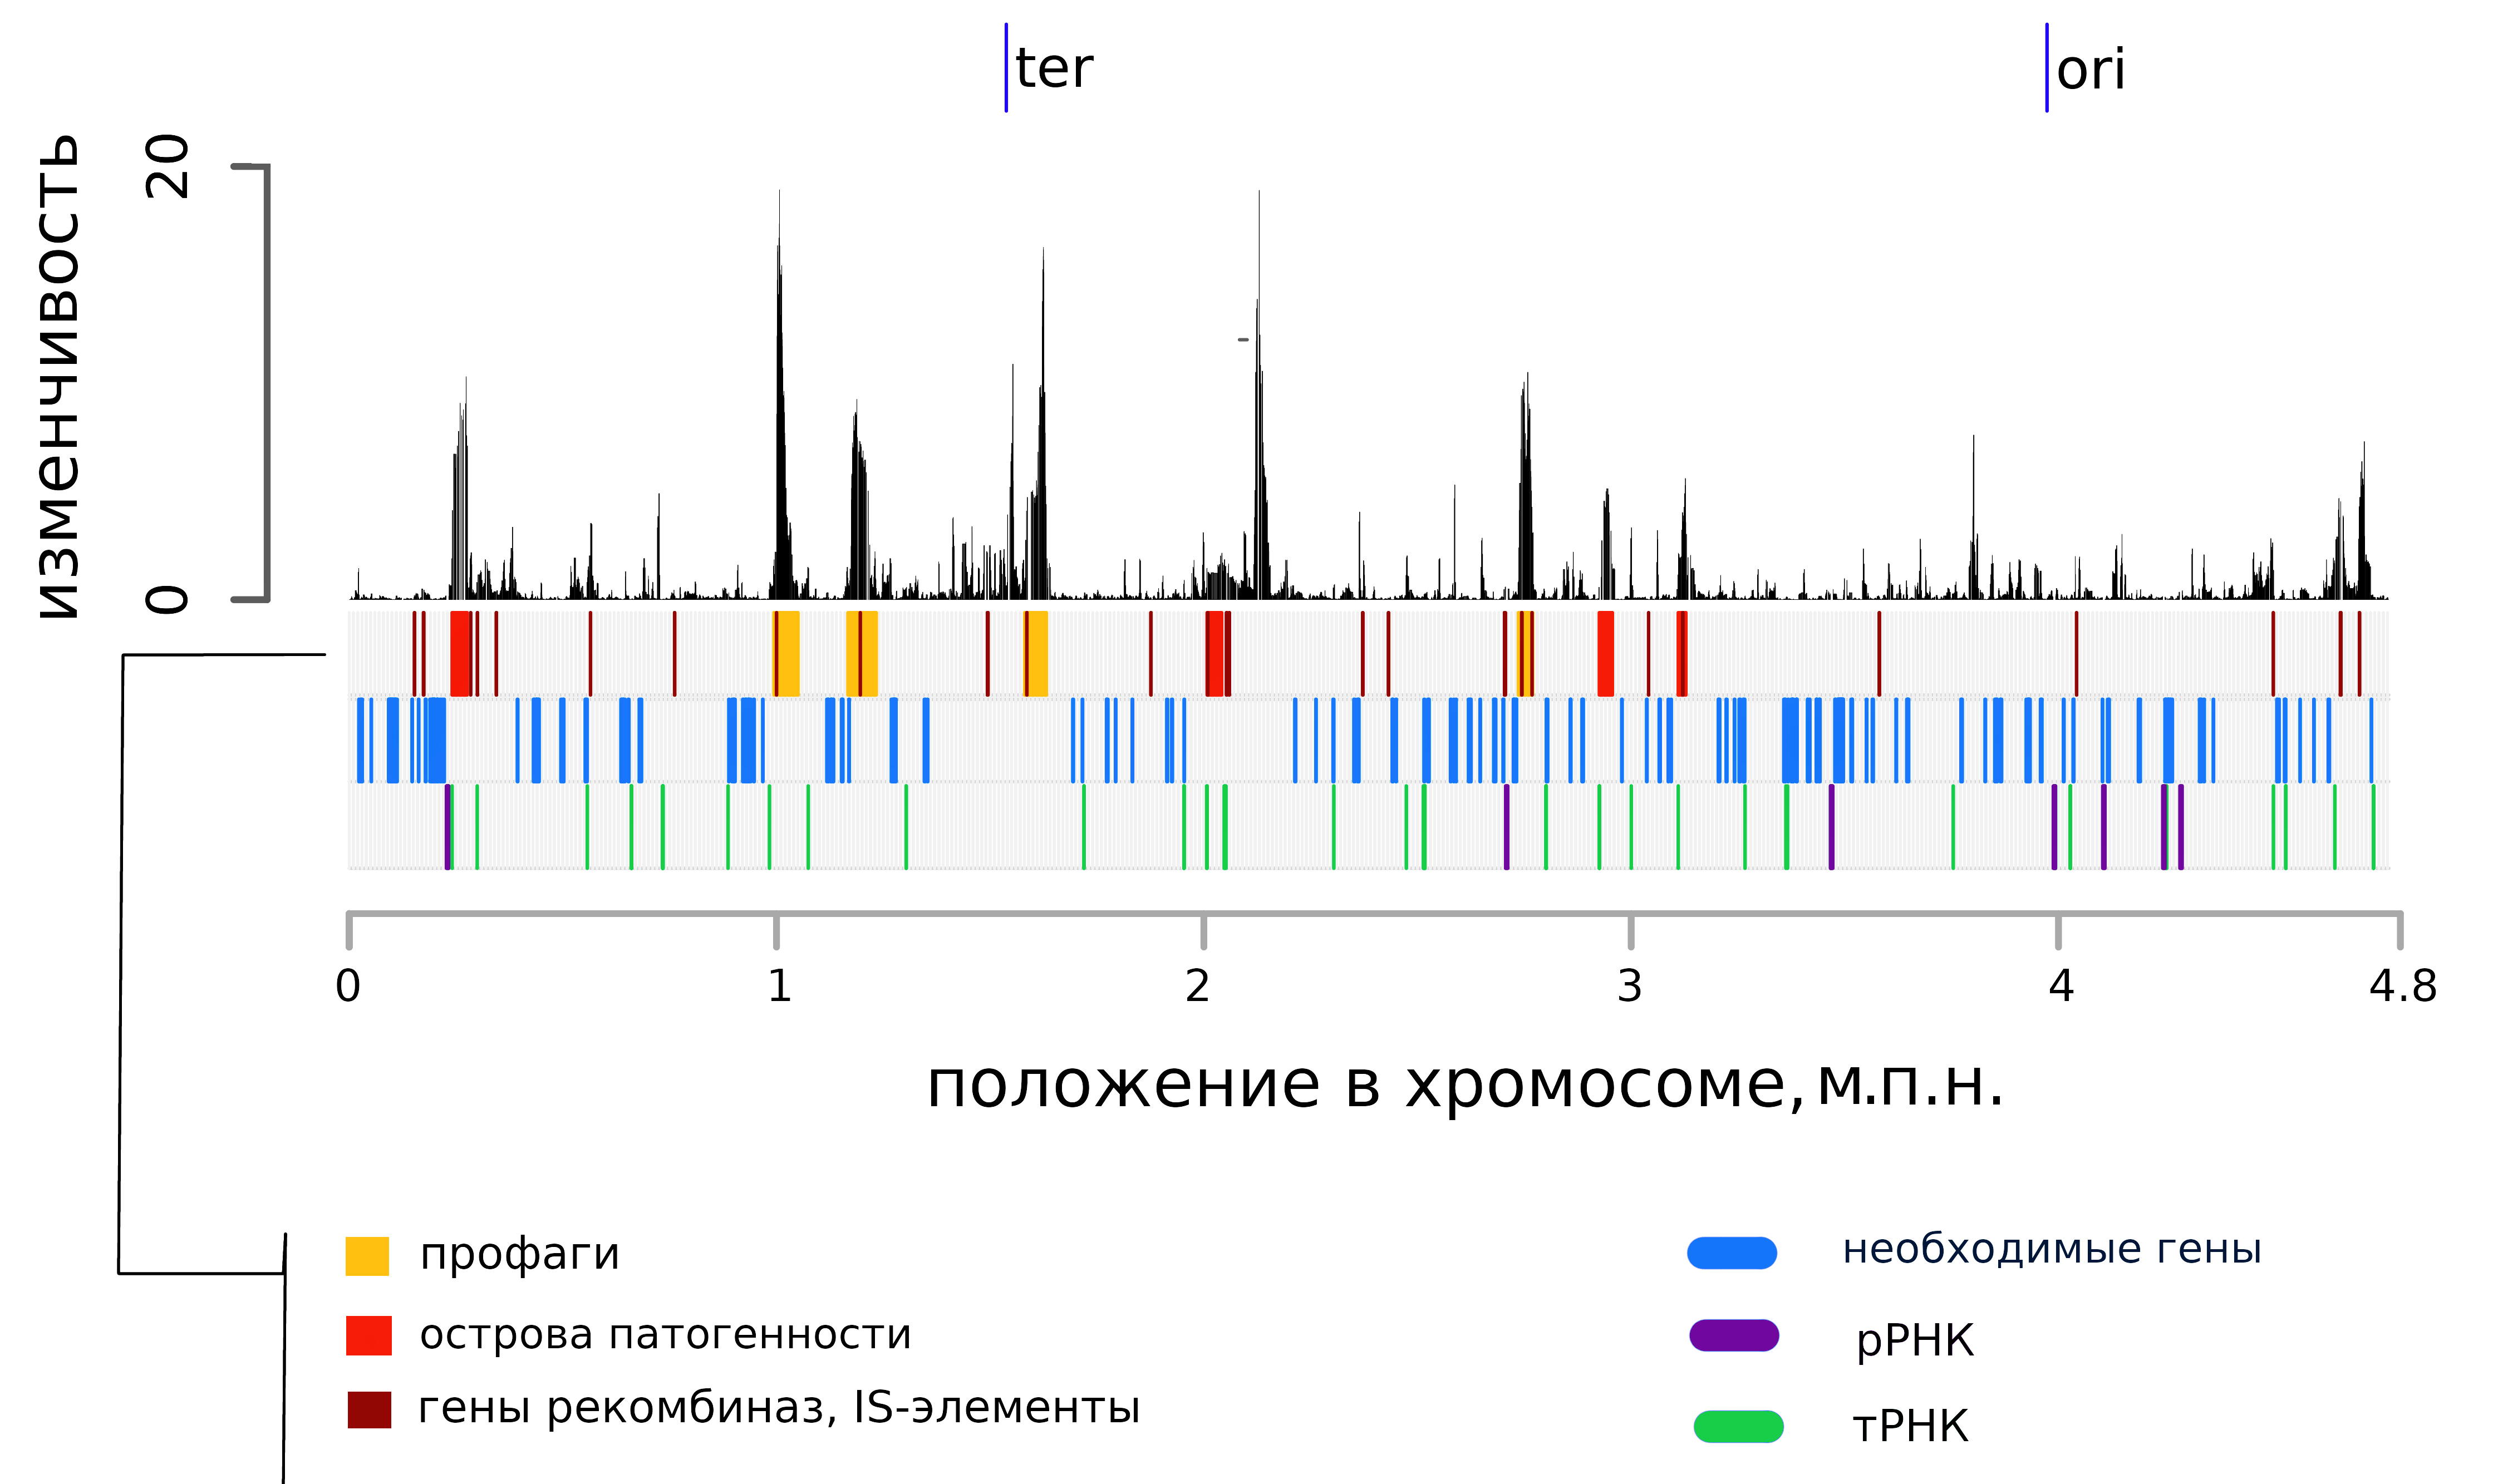
\includegraphics[width=\textwidth]{Dissertation/images/complexity/figure5plus2.png}
  \caption{Профиль вариабельности генома \textit{E. coli LF82}. Цветом обозначены острова патогенности, профаги, гены, ассоциированные с мобильными элементами генома, жизненно-необходимые гены, гены транспортных и рибосомных РНК. Области повышенной изменчивости содержат меньше жизненно-необходимых генов. Профаги и острова патогенности обладают повышенным уровнем изменчивости по сравнению с остальной частью генома.}
  \label{img:complexity_lf82} 
\end{figure}


\subsection{Сравнение профилей вариабельности филогрупп \textit{E. coli}}
Рассмотрим, как соотносятся профили изменчивости геномов из различных внутривидовых структур данного вида. Ценность подобного анализа состоит в возможности установить временную динамику "горячих"\ точек изменчивости (их устойчивость во времени). Также, подобное сравнение является еще одной проверкой предложенного метода: если у геномов из разных подвидовых структур не будет наблюдаться схожести в профиле вариабельности, то это ставит под сомнение ценность анализа для вида в целом. С другой стороны, воспроизводимость --- схожесть профилей --- будет свидетельством того, что получаемый при анализе профиль изменчивости отражает некоторый реальный биологический эффект. 

Для проведения данного анализа мы использовали геномы из пяти наиболее крупных филогрупп (A, B1, B2, D, E) \textit{E. coli}. Мы выбрали по одному референсному геному из каждой филогруппы; для каждого из референсных геномов подобрали 100 наиболее близких (по суммарной ширине выравнивания) геномов, доступных в базе RefSeq, в которой на момент проведения анализа содержалось 5466 геномов кишечной палочки; оценили профиль изменчивости внутри каждой из филогрупп независимо, используя только геномы данной филогруппы. 

\begin{figure}[!ht] 
  \center
    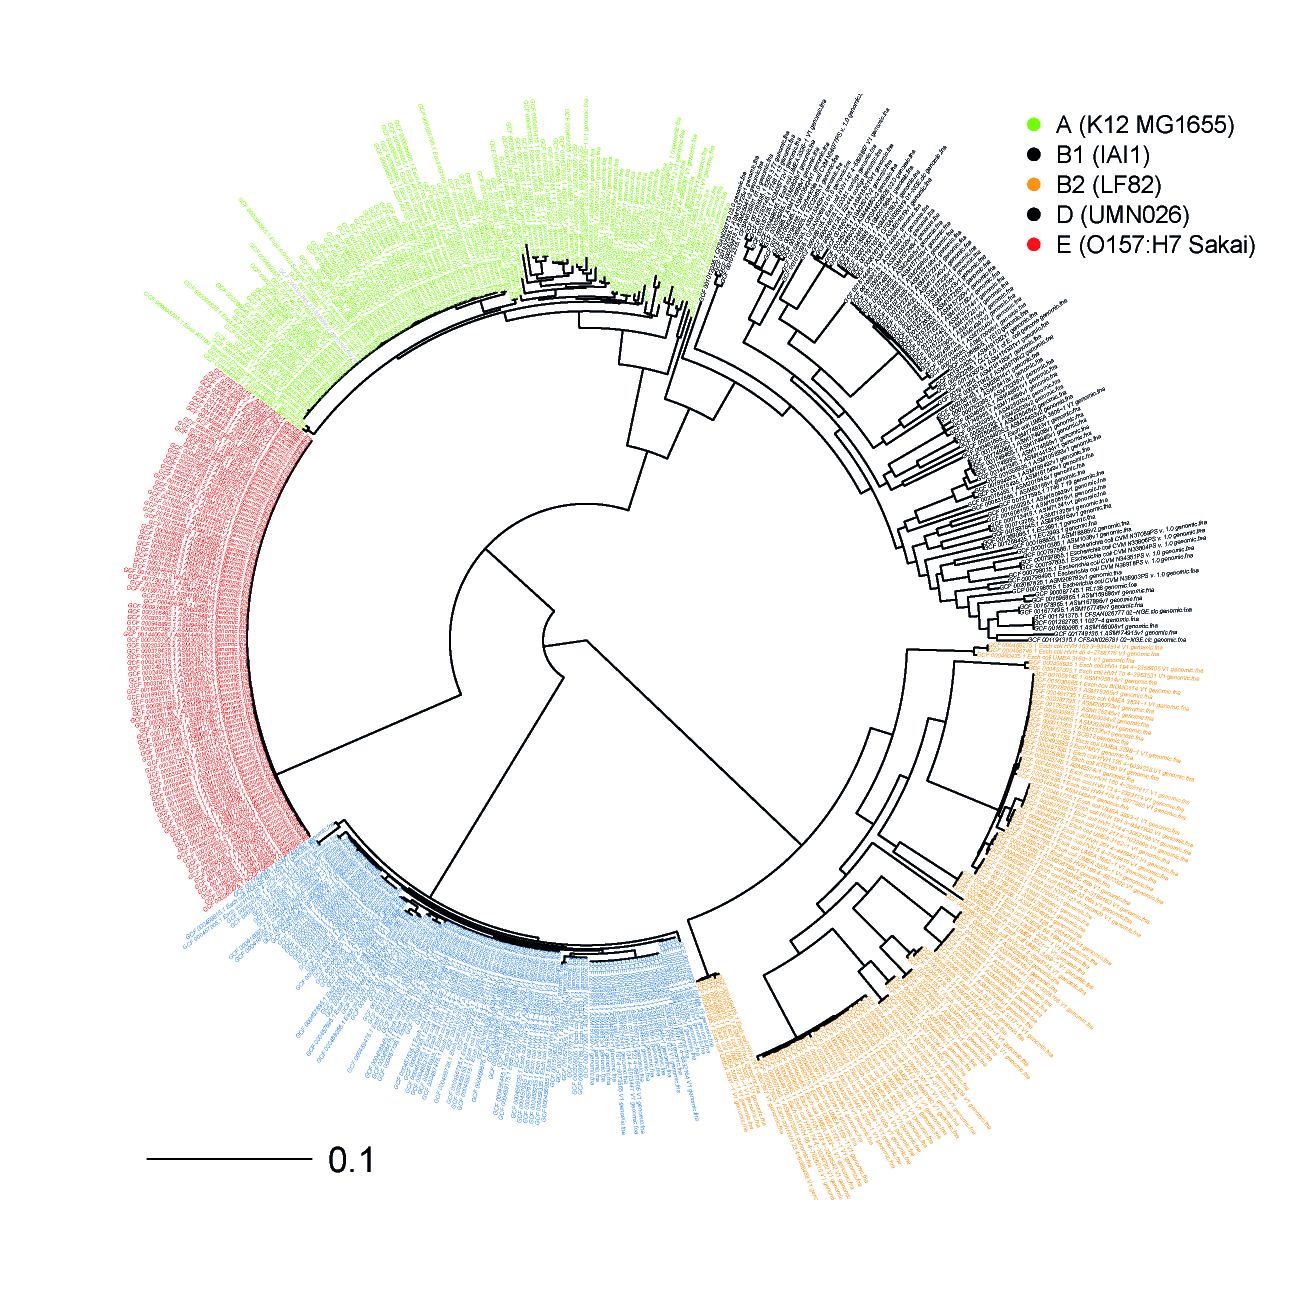
\includegraphics[width=0.65\textwidth]{Dissertation/images/complexity/coli_phylogroups.png}
  \caption{Филогенетическое дерево выборки геномов \textit{E. coli}, состоящей из представителей пяти крупных филогрупп: A, B1, B2, D, E (обозначены зеленым, черным, оранжевым, синим, красным цветом соответственно).}
  \label{img:phylogroups} 
\end{figure}

На рисунке~\ref{img:phylogroups} показано филогенетическое дерево подобранного таким образом набора геномов. На рисунке~\ref{img:phylogroups_complex} показаны профили вариабельности по пяти геномам из различных филогрупп, серым цветом обозначены блоки синтении, оранжевым - области нахождения профагов. Длины геномов значительно различаются: от 4.6 млн. п.о. в случае \textit{K12} до 5.5 м.п.н. у \textit{O157:H7 Sakai}. Профили изменчивости геномов масштабированы таким образом, чтобы они совпадали по длине на рисунке; снизу от профилей изменчивости показаны координатные оси.

\begin{figure}[!ht] 
  \center
    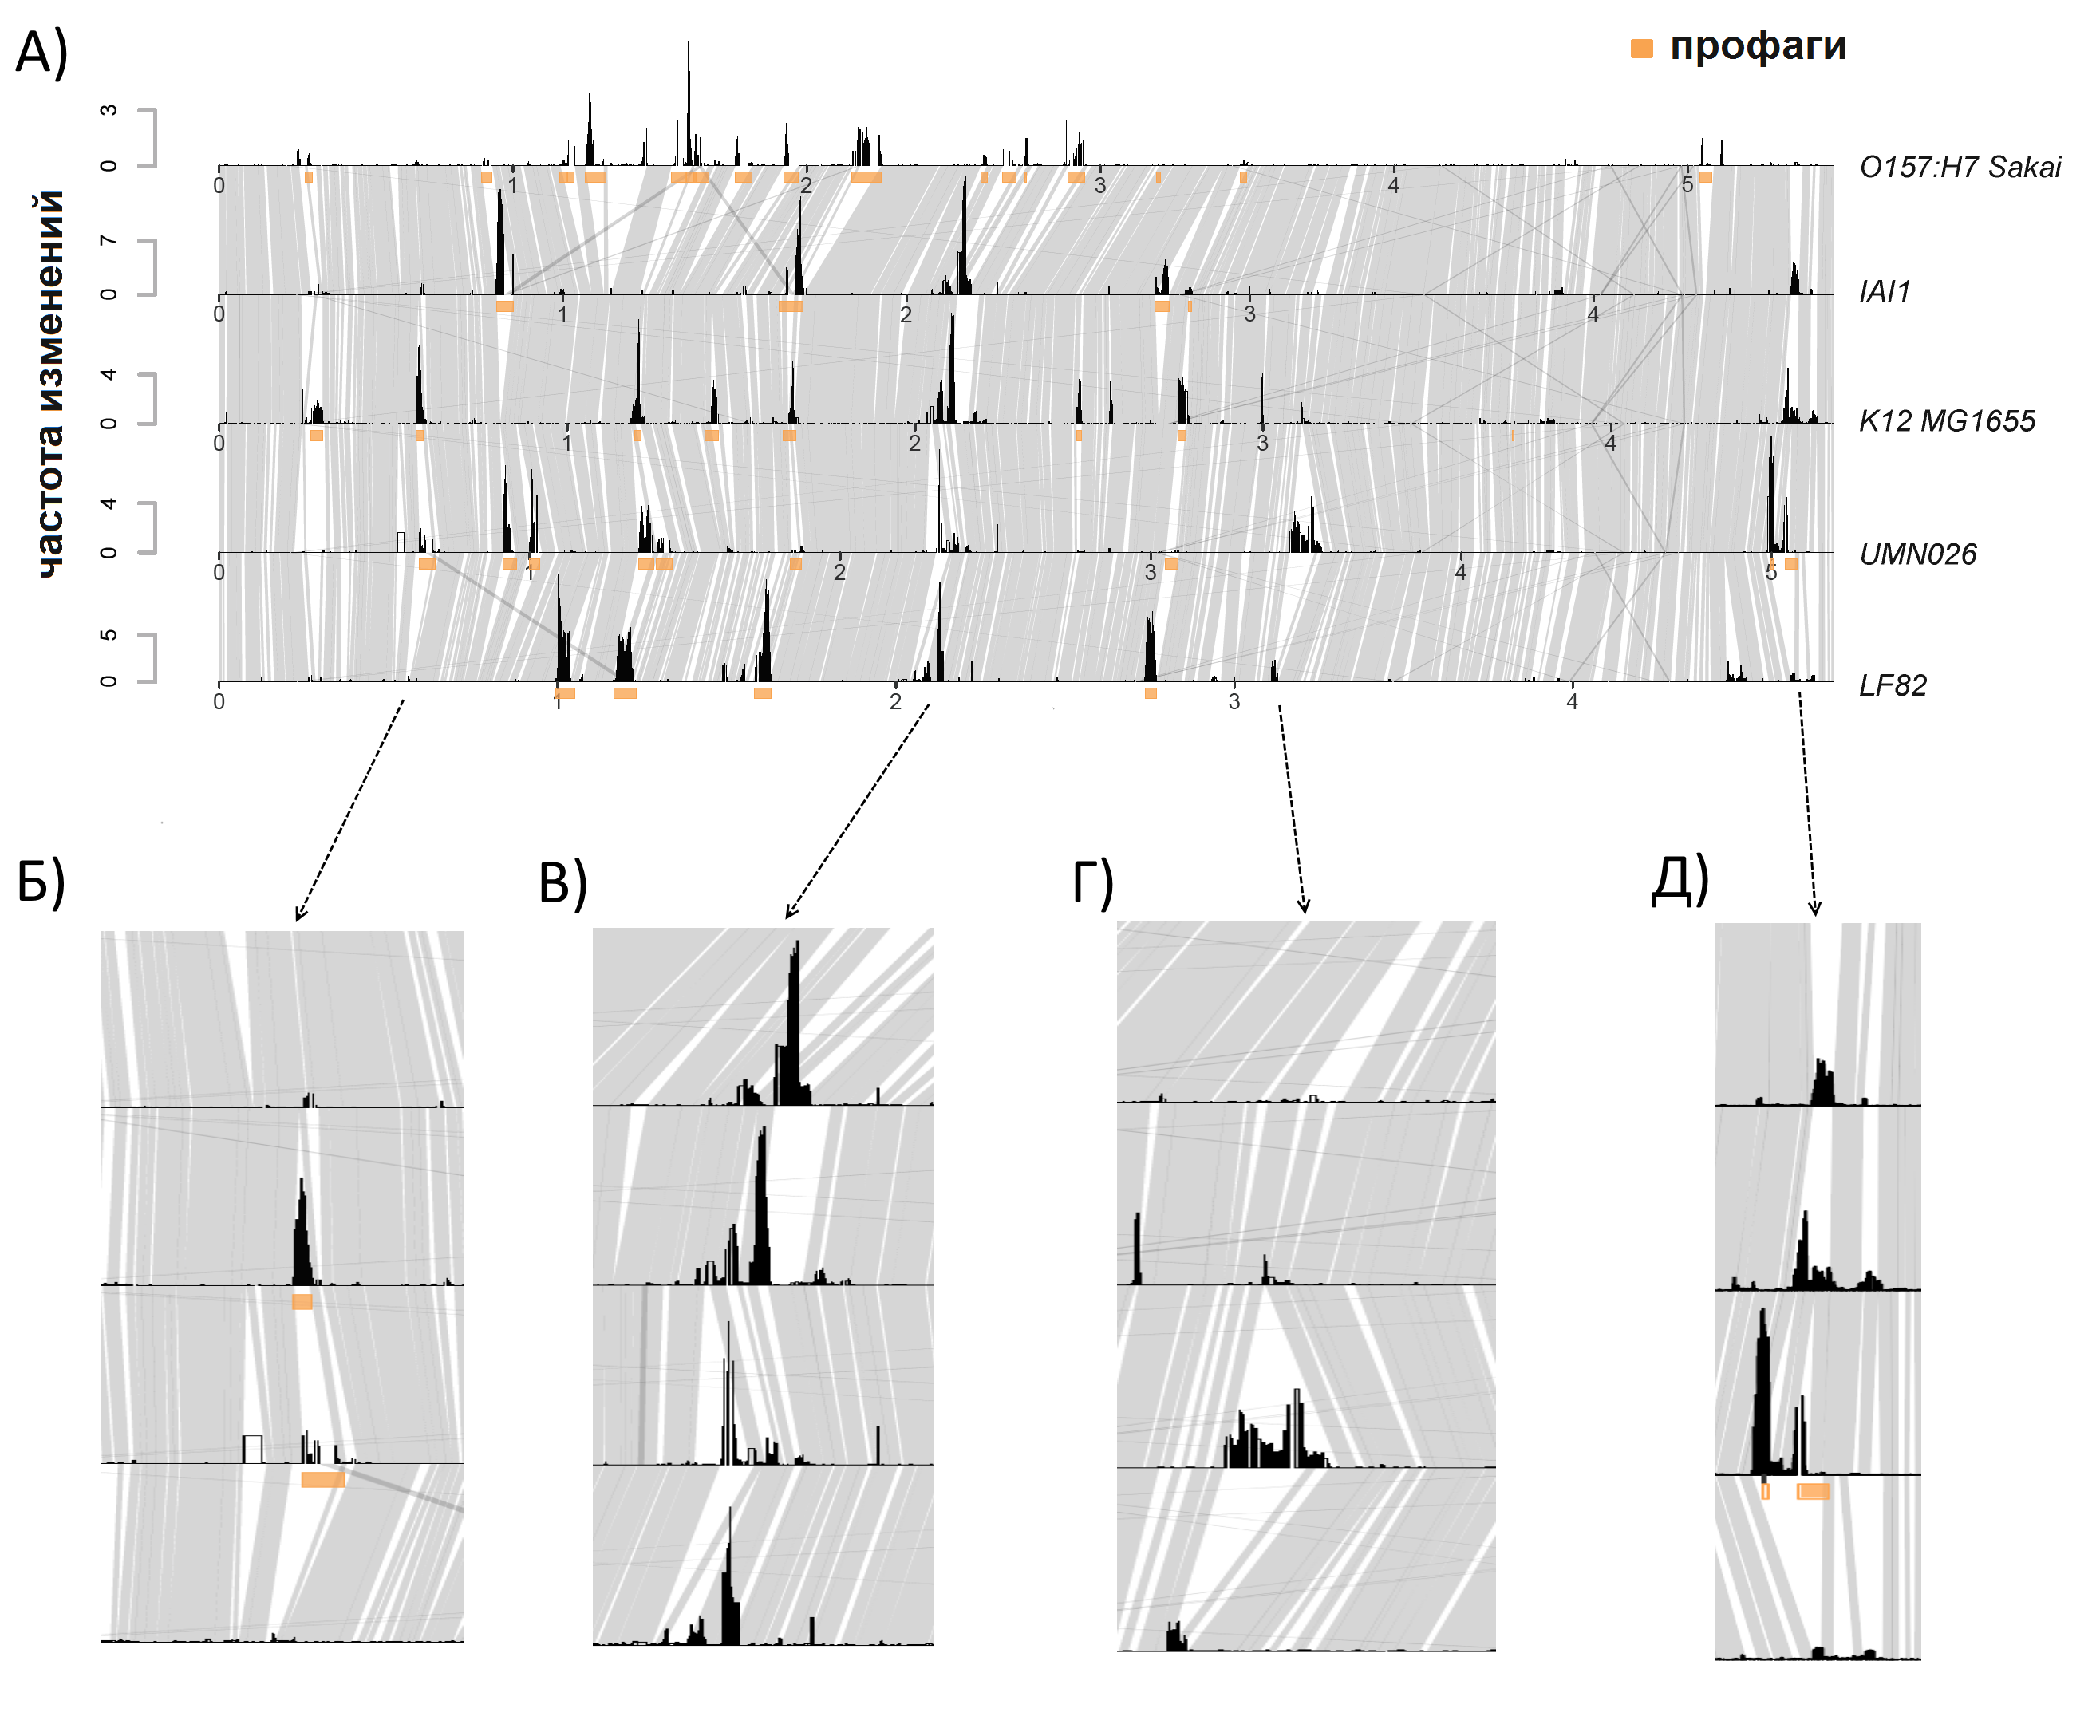
\includegraphics[width=\textwidth]{Dissertation/images/complexity/coli_phylogroups_complexity_3.png}
  \caption{Сравнение профилей вариабельности представителей пяти филогрупп \textit{E. coli LF82}. Оранжевым цветом выделены области, определенные как профаговые. Блоками серого цвета показаны блоки синтении.}
  \label{img:phylogroups_complex} 
\end{figure}

Как и в вышеописанном случае анализа 327 геномов кишечной палочки, анализ по отдельным филогруппам показывает, что большая часть областей с повышенной вариабельностью соответствует местам встройки фагов. Особенно это заметно в случае филогруппы E (штамм \textit{O157:H7 Sakai}), экспансия фагов в которой привела к значительному увеличению размера генома.   

В целом, профили обладают высокой долей сходства: значительная часть областей повышенной вариабельности сохраняет свое расположение у части, либо во всех филогруппах. Это наблюдается как для профаговых областей (рис.~\ref{img:phylogroups_complex} Б), так и для областей без признаков профагов и других мобильных элементов (рис.~\ref{img:phylogroups_complex} В). Горячие точки могут иметь различную степень изменчивости в разных филогруппах (рис.~\ref{img:phylogroups_complex} Б, Г, Д).

Заметно существование "холодных"\ областей генома, обладающих низкой вариабельностью во всех филогруппах. Длина этих низко-вариабельных участков может значительно превышать характерные длины оперонов, и достигать величин порядка миллиона пар оснований (например, область в окрестности 4 млн. п.о. на рисунке~\ref{img:phylogroups_complex} А.

\subsection{Сравнение профилей вариабельности филогрупп у других видов}

В данном разделе мы приводим результаты сравнения профилей изменчивости для филогрупп у других видов бактерий. Мы рассмотрели филогруппы двух видов рода \textit{Pseudomonas} (\textit{P. aeruginosa} и \textit{P. fluorescens}), один из этих видов является естественно-компетентным, а также у \textit{Neisseria gonorrhoeae} - также естественно компетентного вида, для которого характерна высокая частота рекомбинационных событий \cite{yu2014genome}.

\textit{Pseudomonas} - род грамотрицательных бактерий, отдельные виды которого значительно различаются по метаболическому потенциалу и занимаемым экологическим нишам. \textit{P. fluorescens} обитают преимущественно в почве и являются естественно компетентными. \textit{P. aeruginosa} - оппортунистические патогены человека, для которых компетентность наблюдалась лишь в условиях жизни в биопленке \cite{nolan2019pseudomonas}. На рисунке~\ref{img:pseudo_phylogroups} показаны филогенетические деревья для двух видов, цветом выделены клады дерева, отобранные для оценки и сравнения профилей изменчивости. Для \textit{P. fluorescens} в первой кладе было 95 генома, и 115 геномов --- во второй; для \textit{P. fluorescens} в первой кладе было 73 генома и 143 генома --- во второй.

\begin{figure}[!ht] 
  \center
    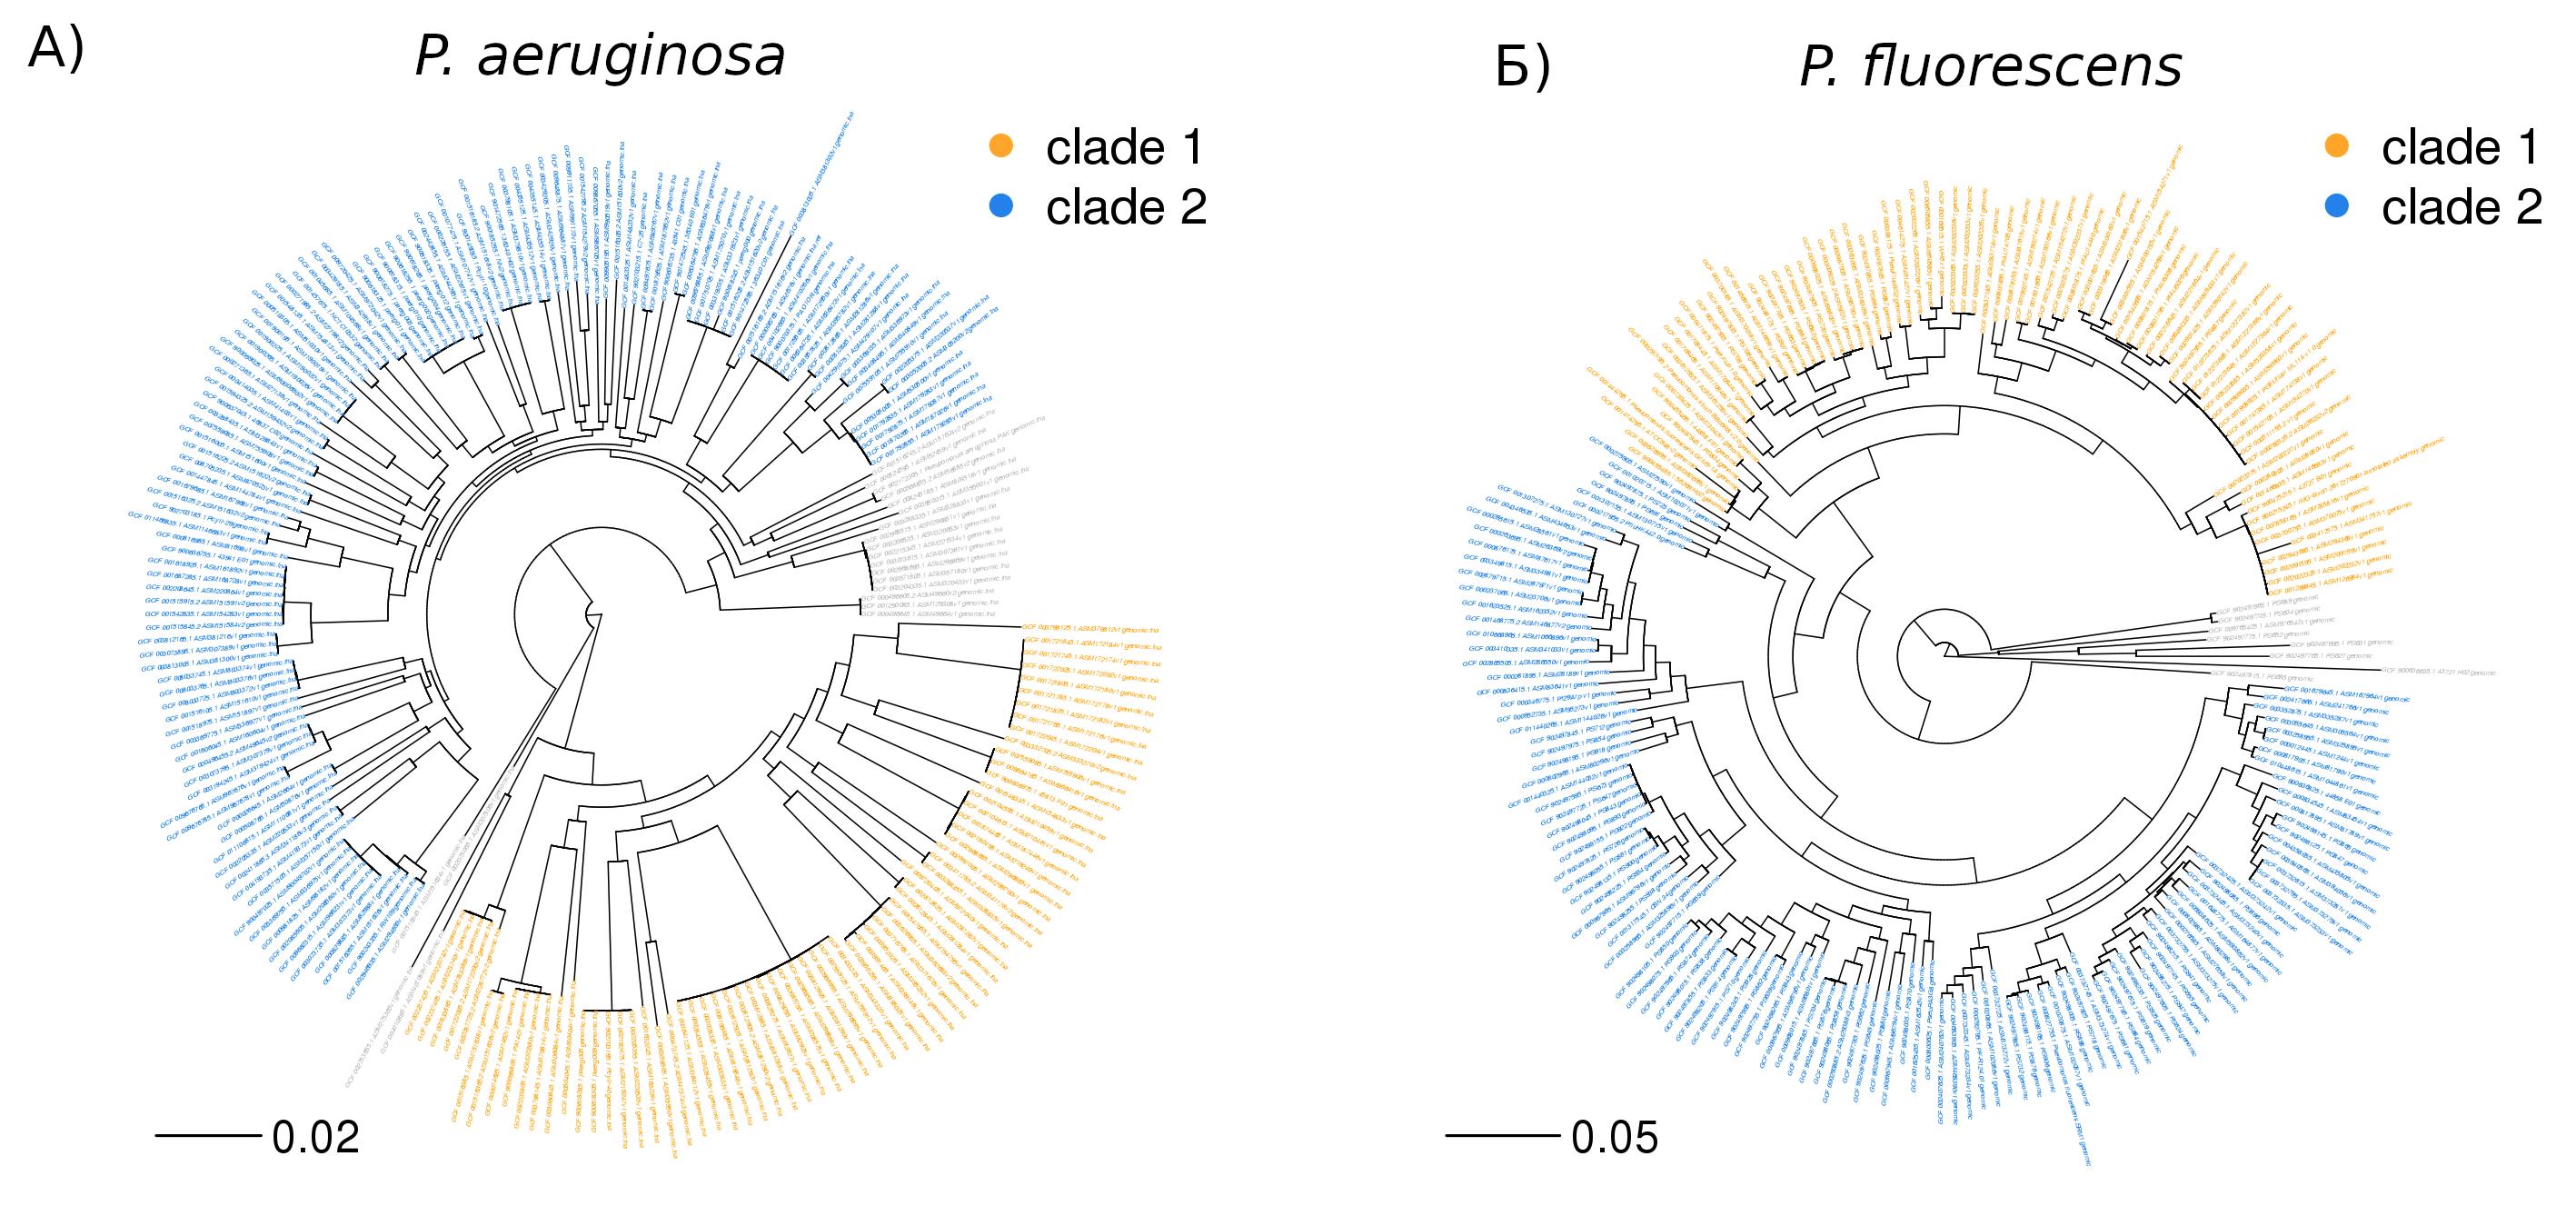
\includegraphics[width=\textwidth]{Dissertation/images/complexity/pseudo_phylogroups.png}
  \caption{Филогенетическое дерево геномов видов: А) \textit{P. aeruginosa} и Б) \textit{P. fluorescens}. Оранжевым и синим цветом выделены клады дерева, отобранные для анализа профилей изменчивости. }
  \label{img:pseudo_phylogroups} 
\end{figure}

На рисунке~\ref{img:pseudo_complexity} показано сравнение профилей изменчивости, оцененных независимо для геномов из различных клад филогенетического дерева. В случае \textit{P. aeruginosa}, подобно \textit{E. coli}, наблюдается значительное сходство профилей изменчивости геномов в двух филогенетических кладах (рис. ~\ref{img:pseudo_complexity} А). В случае \textit{P. fluorescens} подобное сходство выражено слабо и заметно только в небольшом фрагменте ближе к концу хромосомы, после 6 млн. пар оснований, а сами профили вариабельности более равномерны и обладают меньшим количеством выраженных горячих точек (рис. ~\ref{img:pseudo_complexity} Б). Вероятная причина наблюдаемой разницы - высокая частота крупных хромосомных перестроек у \textit{P. fluorescens} (заметно, в том числе, по визуализации блоков синтении). Частые хромосомные перестройки делают анализ локальной изменчивости мало информативным, для применимости метода необходимо: во-первых, наличие локальных участков повышенной изменчивости, и во-вторых, чтобы глобальные перестройки хромосомы происходили сравнительно редко относительно локальных изменений (вставки, делеции и транслокации отдельных генов).

\begin{figure}[!ht] 
  \center
    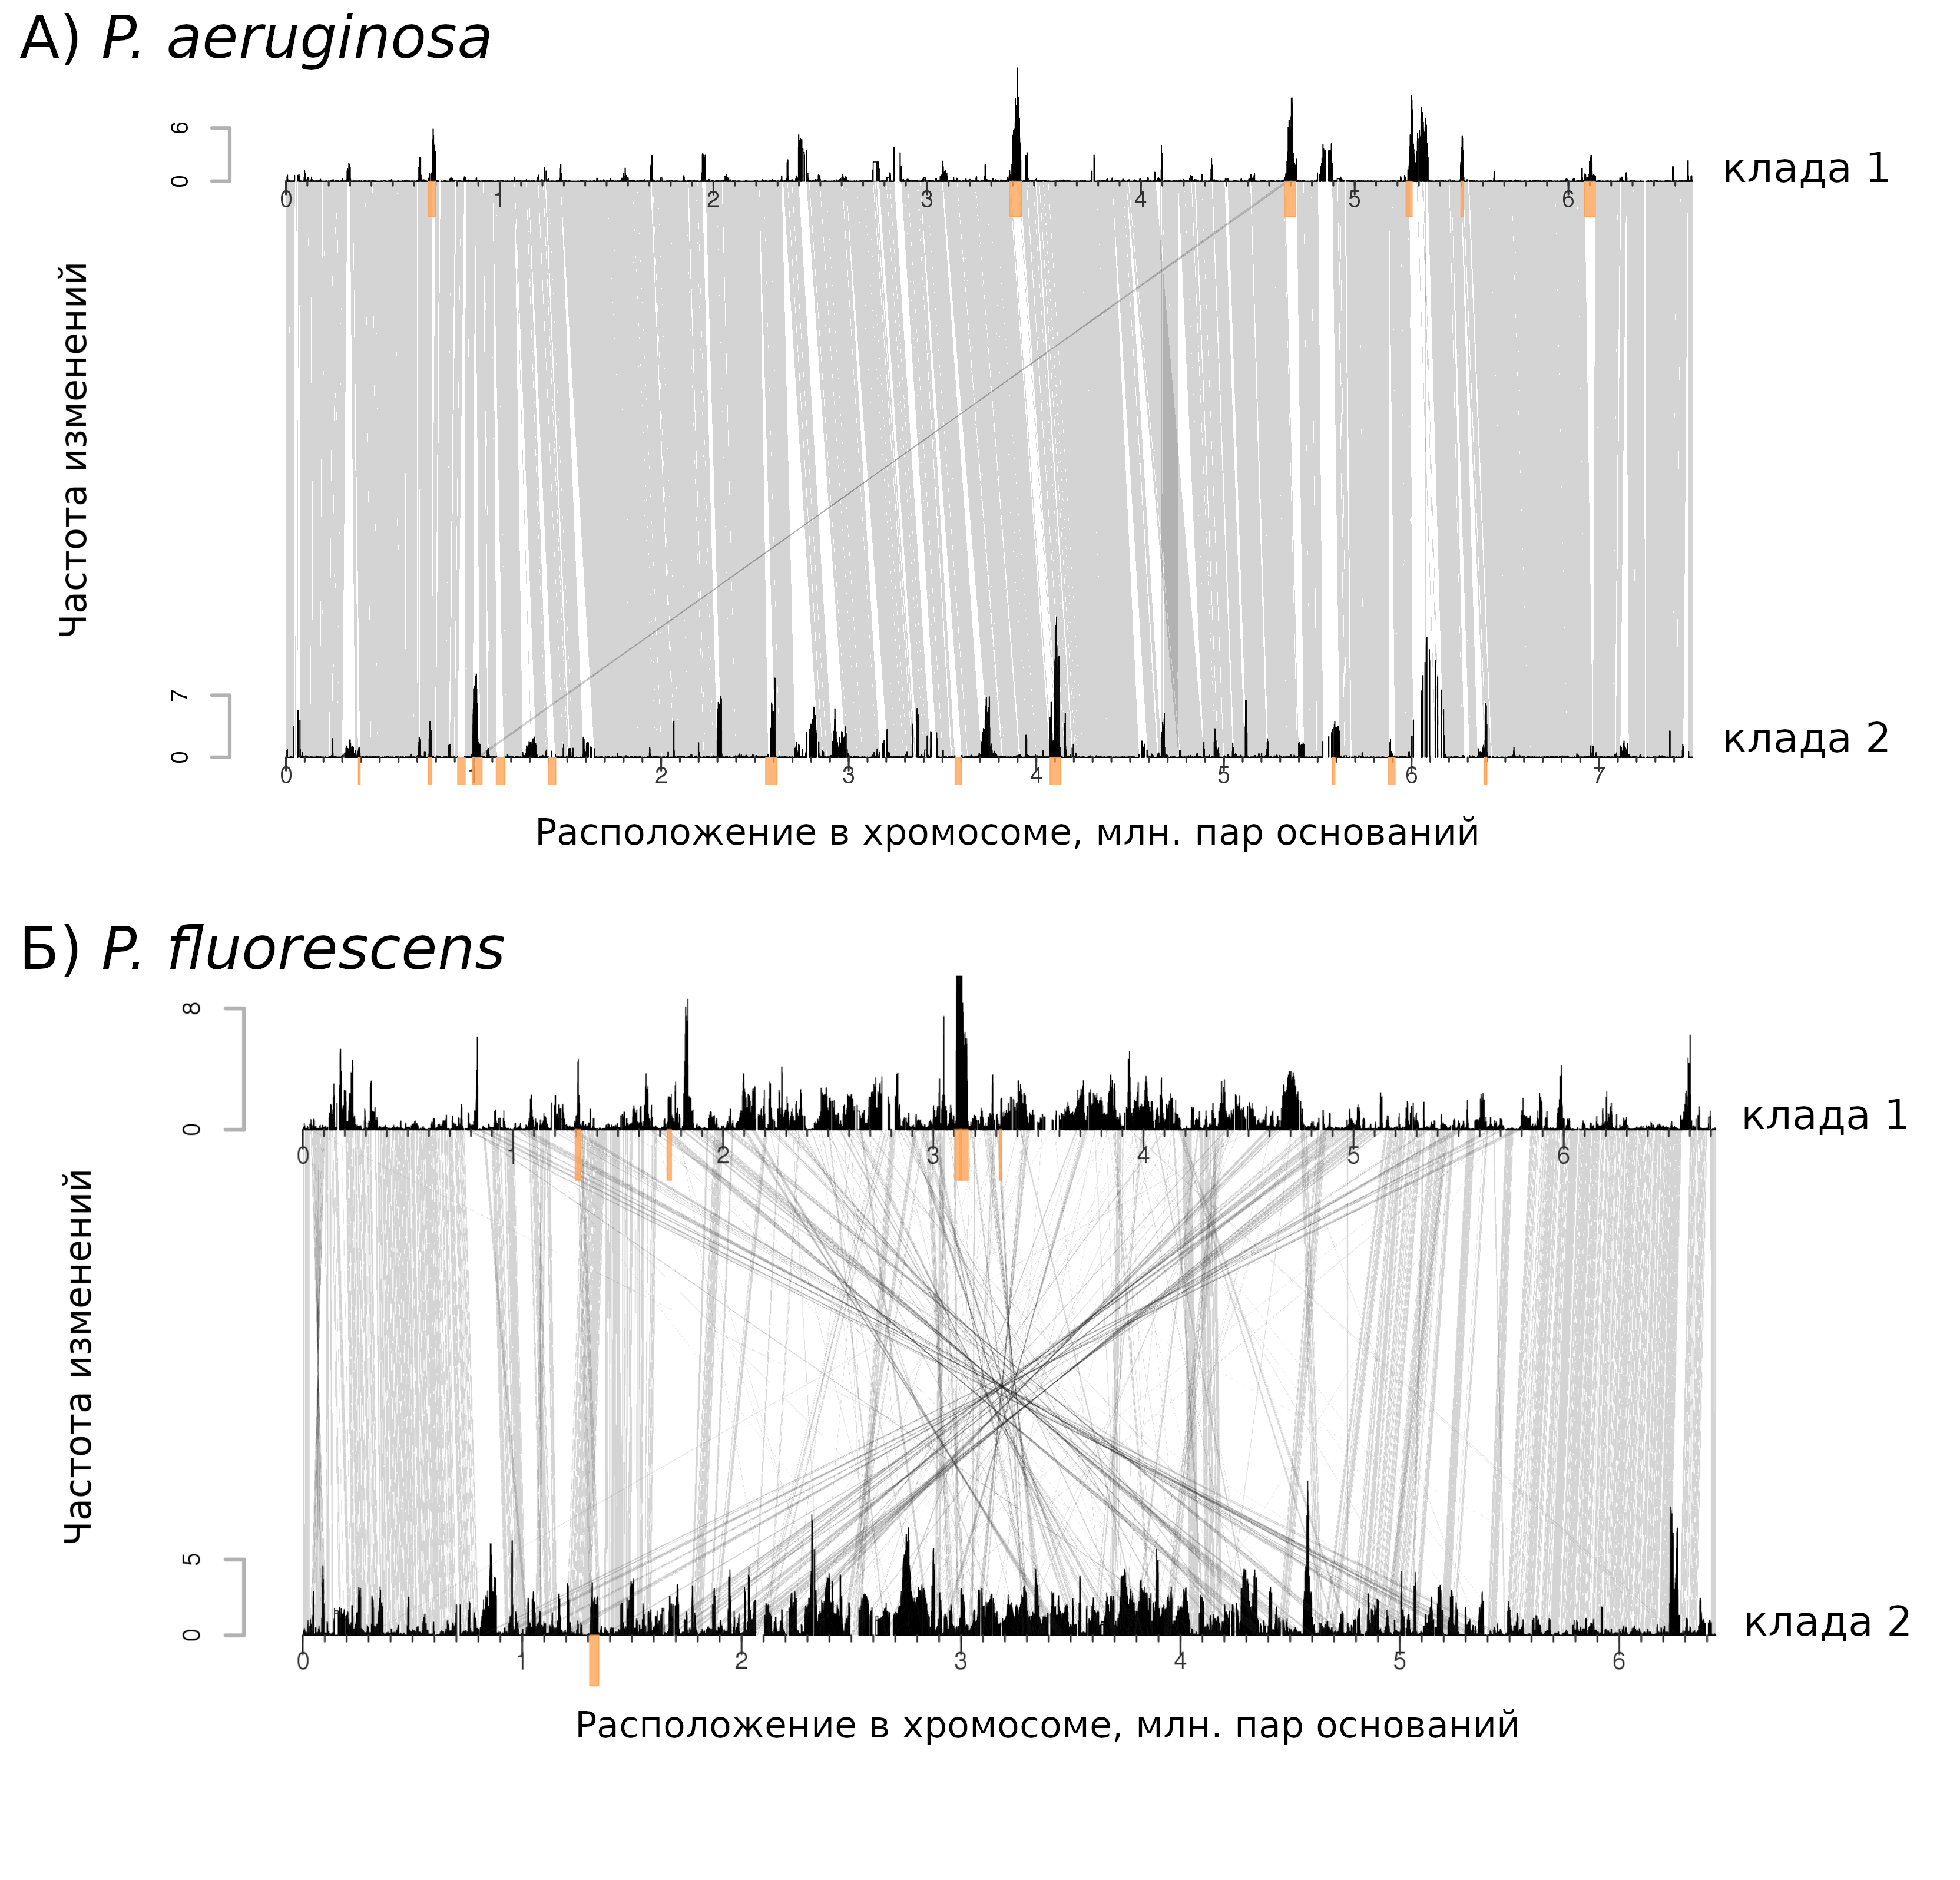
\includegraphics[width=\textwidth]{Dissertation/images/complexity/pseudo_complexity.png}
  \caption{Сравнение профилей вариабельности двух клад вида  А) \textit{P. aeruginosa} и Б) \textit{P. fluorescens}. Оранжевым цветом выделены области, определенные как профаговые.}
  \label{img:pseudo_complexity} 
\end{figure}

Для \textit{N. gonorrhoeae} мы рассмотрели 4 клады. Количество геномов составило 49, 51, 47 и 75 геномов для первой, второй, третьей и четвертой клады, соответственно. Профили геномов из различных клад филогенетического дерева у обладают выским уровнем сходства (рис~\ref{img:ghono_complex}).

\begin{figure}[!ht] 
  \center
    \subcaptionbox{}{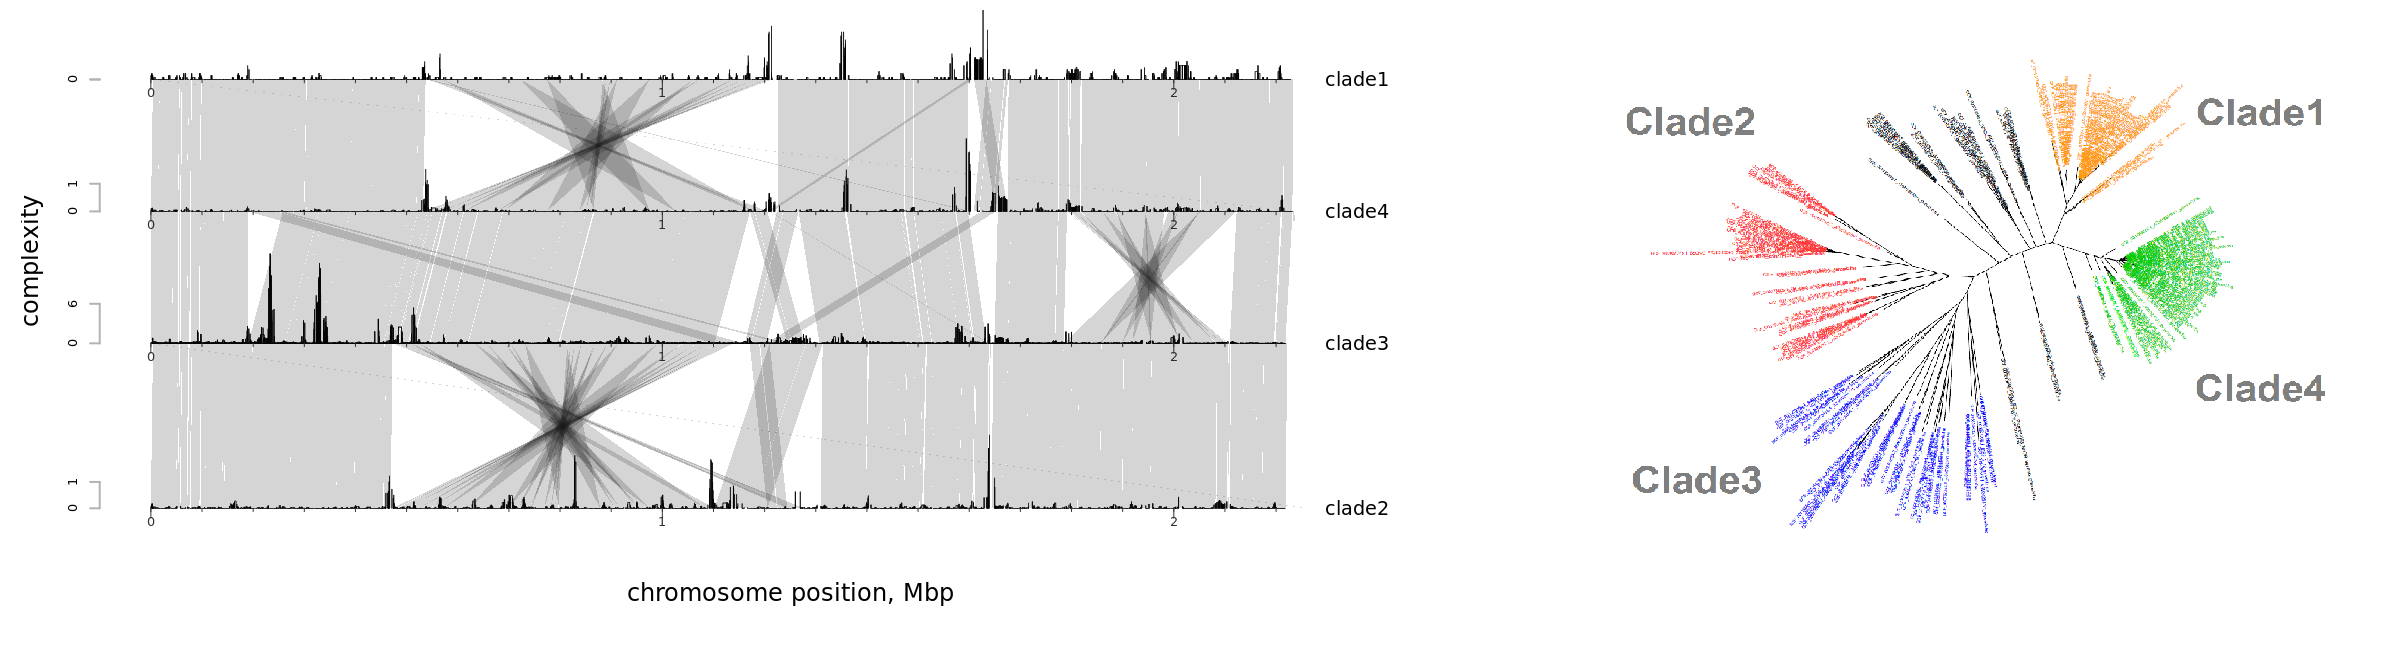
\includegraphics[width=0.6\textwidth]{Dissertation/images/complexity/neisseria_clades.png}}
    \subcaptionbox{}{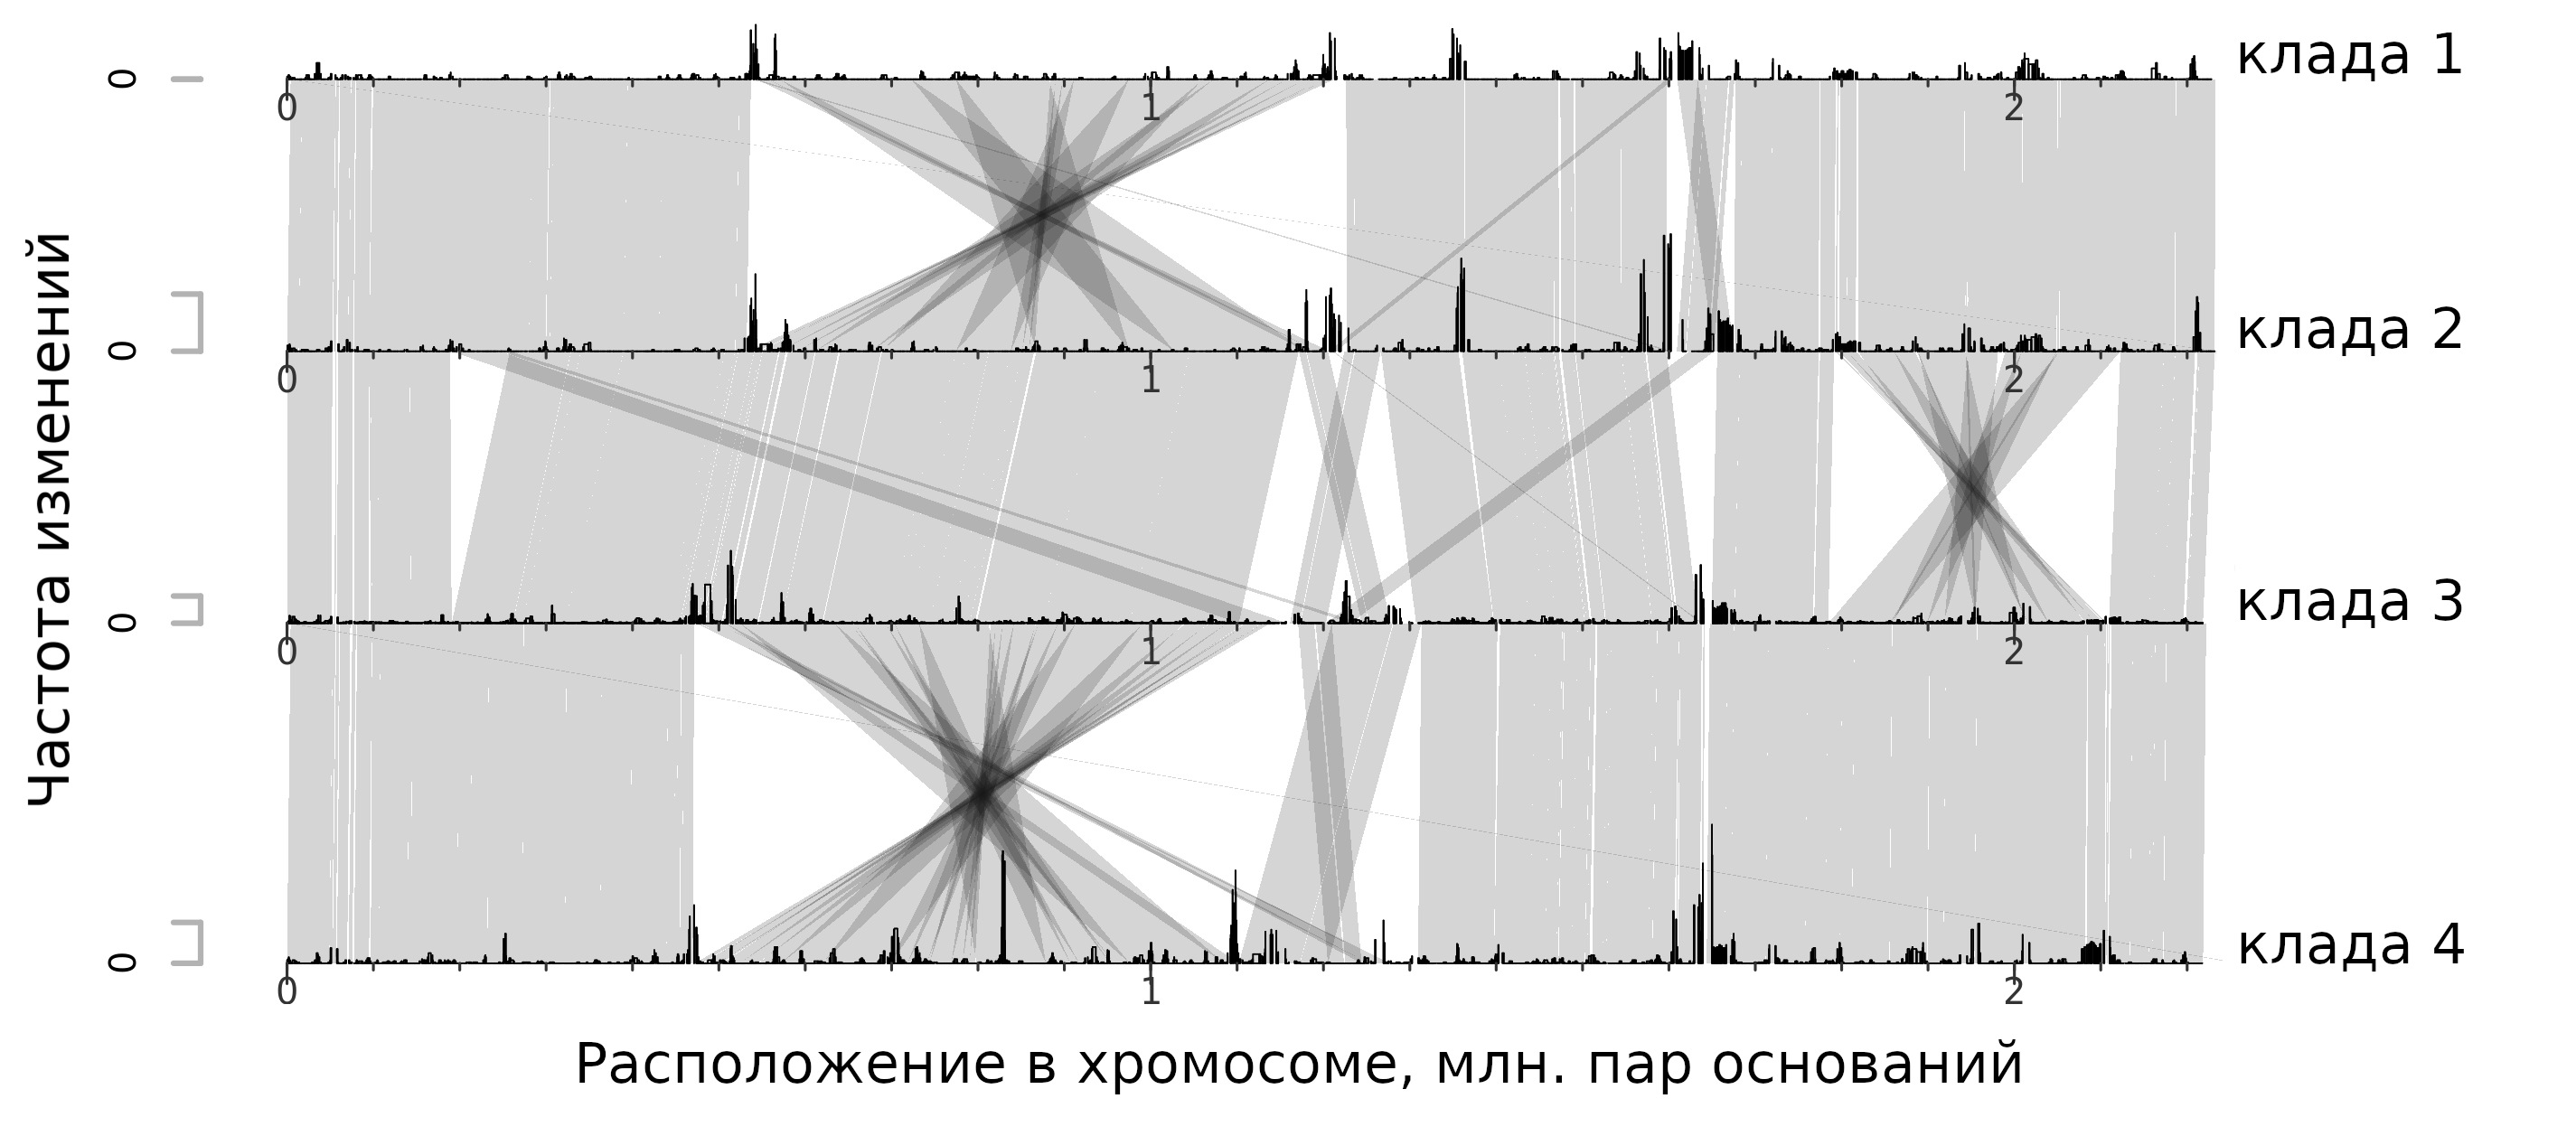
\includegraphics[width=\textwidth]{Dissertation/images/complexity/neisseria_ghono.png}}
  \caption{Сравнение профилей вариабельности четырех филогенетических клад вида \textit{N. gonorrhoeae}. А) Филогенетическое дерево с указанием выбранных клад. Б) сравнение профилей вариабельности.}
  \label{img:ghono_complex} 
\end{figure}

\subsection{Сравнение профилей вариабельности между близкородственными видами}

\begin{figure}[!ht] 
  \center
    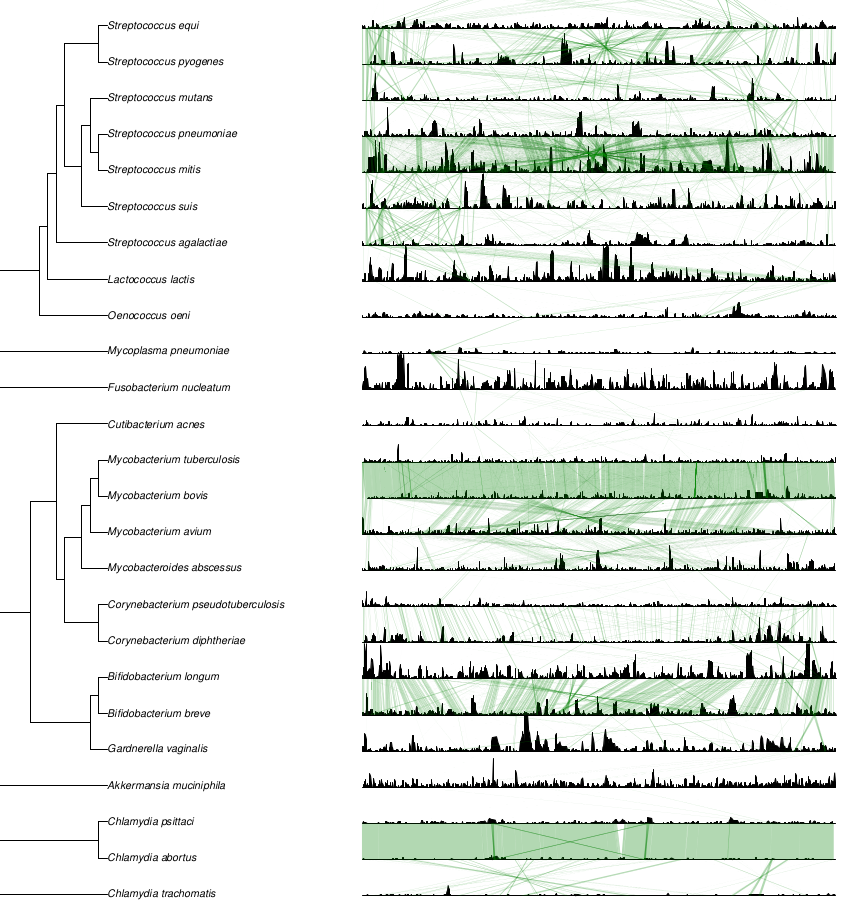
\includegraphics[width=\textwidth]{Dissertation/images/complexity/tree_fragment.png}
  \caption{Фрагмент визуализации профилей изменчивости геномов различных видов. Профили расположены в соответствии с филогенетическим деревом видов, блоки синтении показаны для смежных по дереву видов.}
  \label{img:tree_fragment} 
\end{figure}


\begin{figure}[!ht] 
  \center
    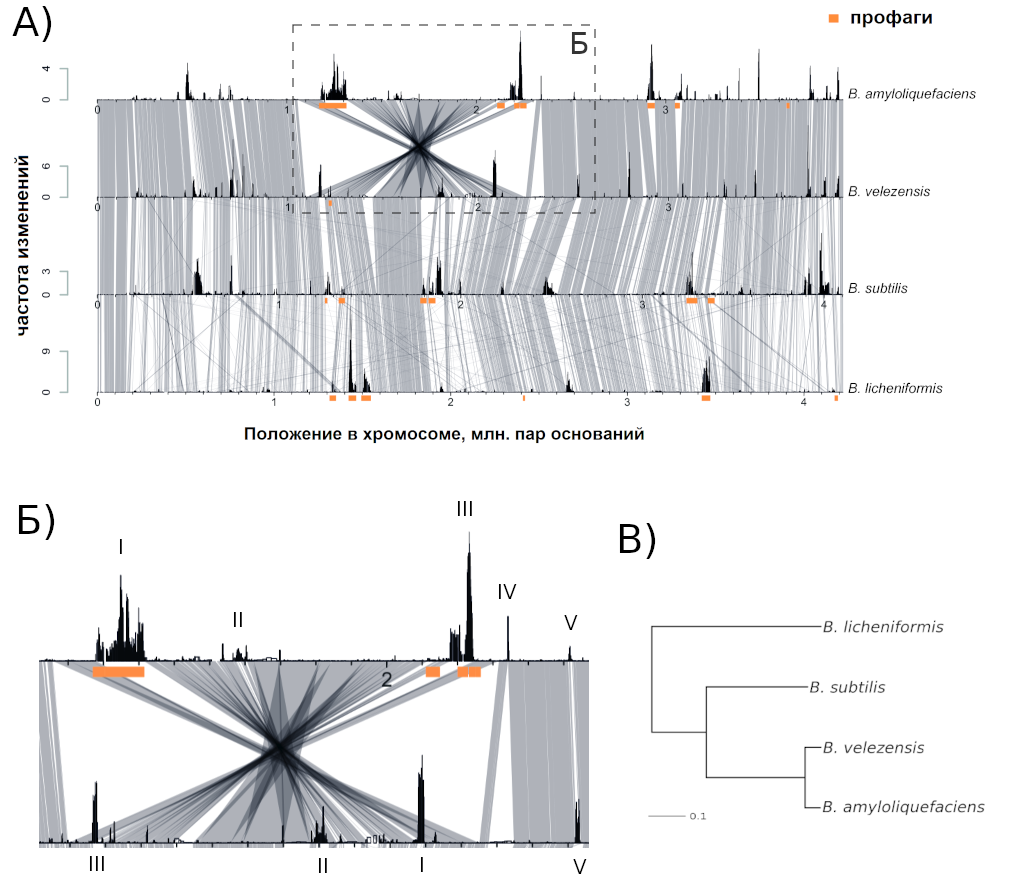
\includegraphics[width=\textwidth]{Dissertation/images/complexity/bacillus_compare_v3.png}
  \caption{Сравнение профилей вариабельности четырех различных видов рода \textit{Bacillus}. А) Профили изменчивости и блоки синтении, оранжевым цветом выделены области, определенные как профаговые, рамка из штрихованных линий показывает фрагмент, представленный на Б). В) Филогенетическое дерево рассматриваемых видов.}
  \label{img:species_complex_bacillus} 
\end{figure}


\begin{figure}[!ht] 
  \center
     \subcaptionbox{}{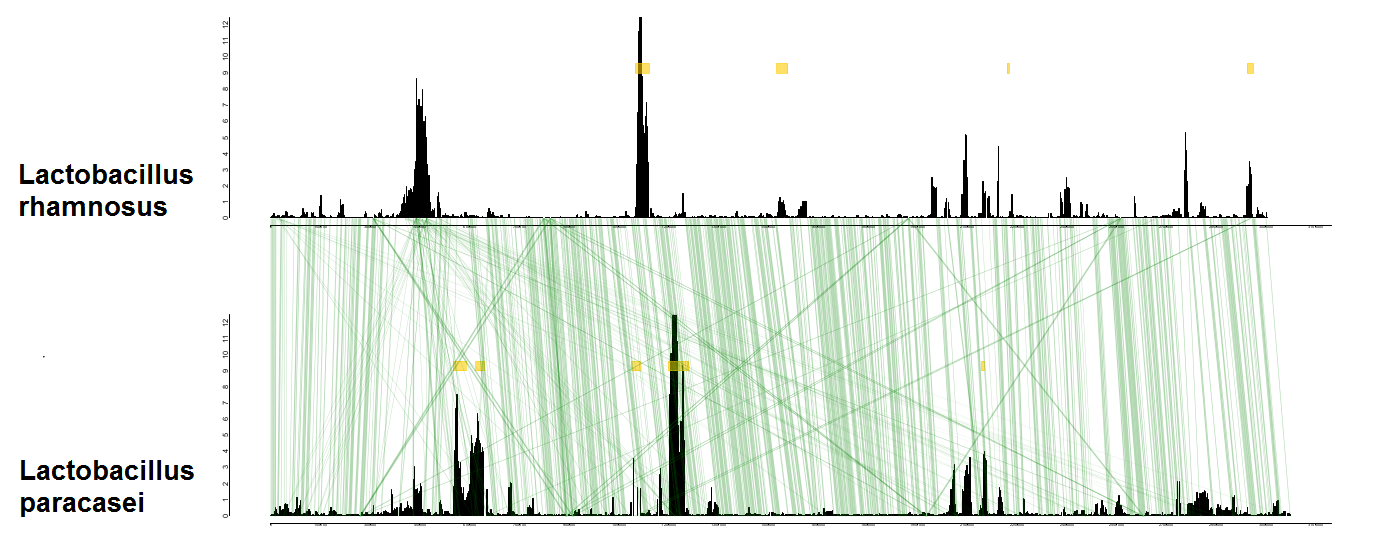
\includegraphics[width=\textwidth]{Dissertation/images/complexity/lacto_complexity.png}}
     \subcaptionbox{}{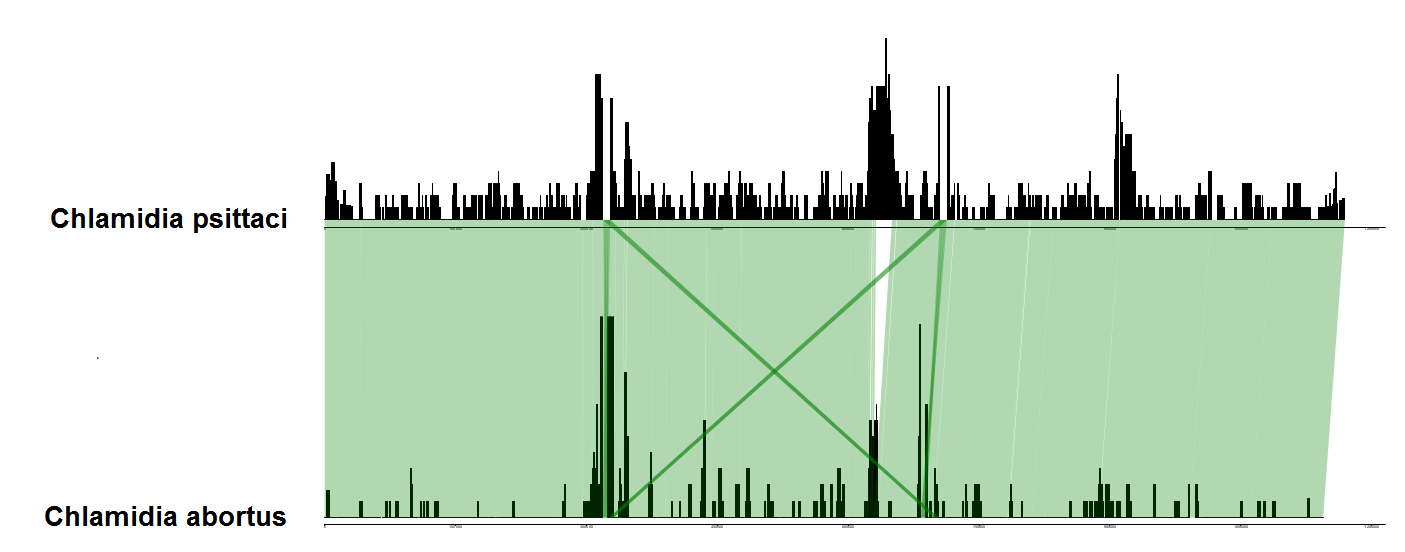
\includegraphics[width=\textwidth]{Dissertation/images/complexity/chlamidia_complexity.png}}
  \caption{Сравнение профилей вариабельности для: А) двух видов рода \textit{Lactobacillus}, Б) двух видов рода \textit{Chlamidia}. Оранжевым цветом выделены области, определенный как профаговые.}
  \label{img:species_complex_lactobacillus_chlam} 
\end{figure}

Внутри вида профили изменчивости обладают высокой степенью сходства. Для выяснения степени сходства профилей изменчивости для геномов из разных видов, мы провели анализ изменчивости у 143 видов бактерий и архей. В рассмотрение мы брали те виды, для которых было доступно как минимум 50 геномов на момент начала анализа (2016 год). Визуализация профилей доступна на веб-сервере \url{gcb.rcpcm.org}, о котором будет подробнее рассказано ниже. Все профили изменчивости были расположены в соответствии с филогенетическим деревом, блоки синтении рассчитывались между всеми парами видов, расположенными последовательно на дереве. Фрагмент итоговой визуализации показан на рисунке~\ref{img:tree_fragment}, полная визуализация доступна по адресу \url{https://github.com/paraslonic/GCB_revision/blob/master/figures/S3_Fig.pdf}. 

В большинстве случаев, когда между видами наблюдается малое количество геномных перестроек, профили изменчивости похожи (горячие точки находятся в схожем окружении). Ниже, для примера, мы приводим отдельные сравнения профилей изменчивости.

На рисунке~\ref{img:species_complex_bacillus} А показано сравнение профилей изменчивости четырех видов рода \textit{Bacillus}, филогенетическое дерево для рассмотренных видов показано на рисунке~\ref{img:species_complex_bacillus} В. У геномов видов \textit{B. amyloliquefaciens} и \textit{B. velezensis} заметна крупная инверсия (рис.~\ref{img:species_complex_bacillus} А, выделена рамкой), при этом, области высокой изменчивости сохранили свою активность  (рис~\ref{img:species_complex_bacillus} Б, пики изменчивости обозначены римскими цифрами). 

На рисунке~\ref{img:species_complex_lactobacillus_chlam} показано сравнение профилей изменчивости для двух видов лактобацилл и двух видов хламидий.



%\subsection{Разные виды имеют разный характер распределения интенсивности вариабельности вдоль генома}

%Рассмотрим сравнение профилей вариабельности посчитанных для множества различных видов. Как видно из рисунка ...




% ################################################################### HIC 
\section{Связь между уровнем изменчивости и характеристиками генома}\label{chaptComplexWithSMTH}

Профили изменчивости для геномов из различных филогрупп и близкородственных видов показали значительную степень сходства: наблюдается множество "горячих"\ точек изменчивости со стабильным положением в хромосоме. Открытым остается вопрос о причинах этого постоянства положения зон вариабельности, а также факторов определяющих их возникновение, рост либо снижение активности. Ниже мы приводим результаты сравнения между профилем изменчивости и расположением сайтов Chi, а также частотой межхромосомных контактов. 

\subsection{Связь с распределением сайтов Chi.}
Процесс горизонтального переноса генов подразумевает проведение одного из типов рекомбинации. Как было отмечено в обзоре литературы, у бактерии \textit{E. coli} описаны сайты Chi, играющие важную роль в инициации процесса гомологичной рекомбинации. 
На рисунке~\ref{img:chi_lf82} А показан уровень локальной вариабельности и локализация Chi-сайтов для хромосомы штамма \textit{E. coli LF82}. Из приведенного рисунка видно неравномерное распределение сайтов Chi по реплихорам хромосомы и их сниженная представленность в местах локализации профагов/островов патогенности, а также в областях с высокой вариабельностью. На рисунке~\ref{img:chi_lf82} б) показано сравнение уровня вариабельности и расстояний до ближайшего сайта Chi (на соответствующей цепи, лидирующей для правой реплихоры, и отстающей - для левой). Корреляция между уровнем вариабельности и расстоянием до ближайшего Chi-сайта значима (p-value < 1e-16), но значение коэффициента корреляции невелико и составляет 0.25.
% code: /data11/bio/operonTravel/coli/chi/ver3
\begin{figure}[!ht] 
  \center
    \subcaptionbox{}{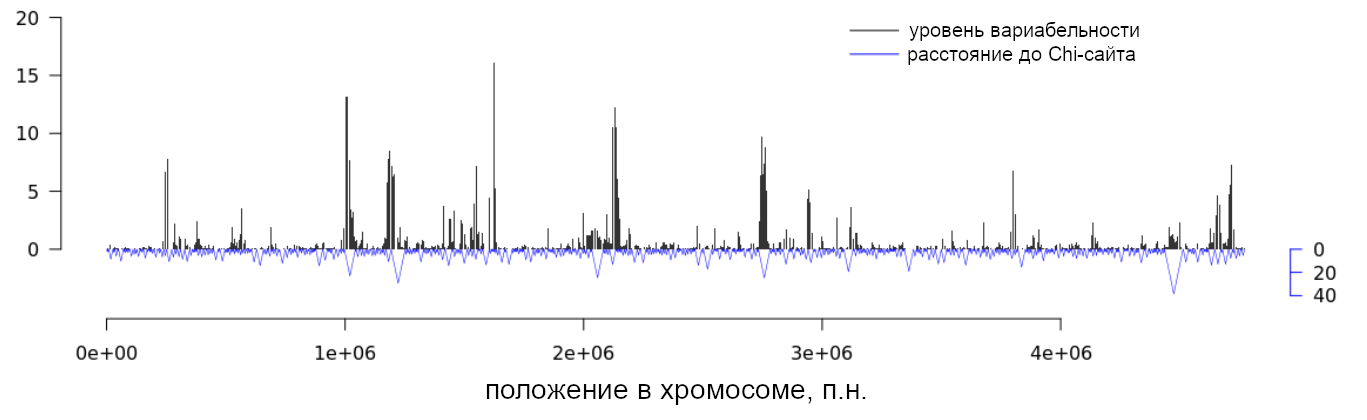
\includegraphics [width=1\textwidth] {Dissertation/images/complexity_with_smth/lf82_chi_sites.png}}
    
    \subcaptionbox{}{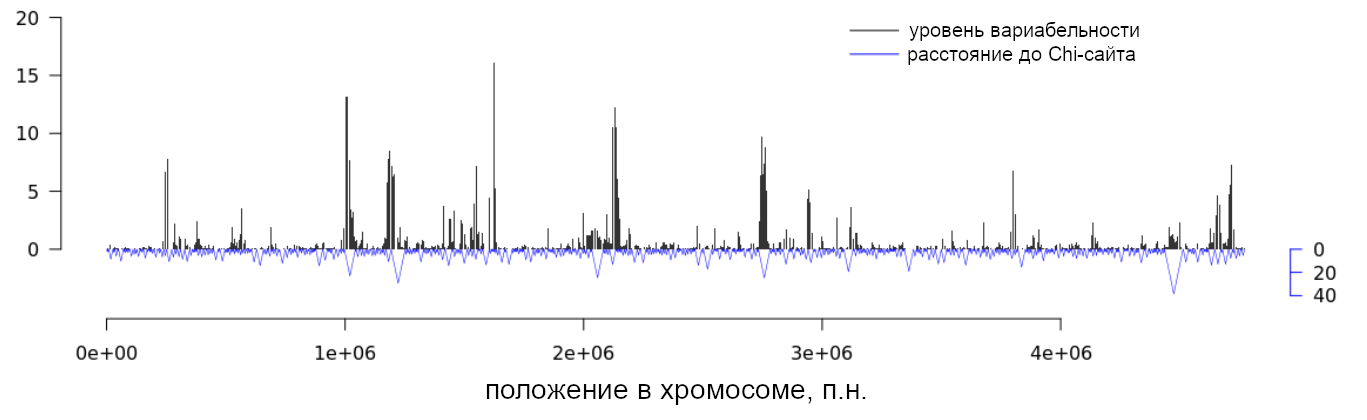
\includegraphics [width=1\textwidth] {Dissertation/images/complexity_with_smth/chidist_complexity.png}}
    
    \caption{Уровень вариабельности и локализация сайтов Chi на двух цепях хромосомы \textit{E. coli LF82}. А) Синие вертикальные линии показывают расположение сайтов Chi на двух цепях хромосомы. Вертикальные пунктирные линии показывают границы реплихор (места начала и конца репликации). Желтым и красным цветом обозначены области расположения профагов и островов патогенности соответственно. Б) Черной линией показан уровень вариабельности, синей - расстояние до ближайшего сайта Chi (в масштабе тысяч пар оснований).}
    \label{img:chi_lf82}
\end{figure}

Эффект более низкой представленности сайтов Chi в горизонтально перенесенных фрагментах был описан ранее\cite{halpern2007identification}. Вероятно, связь между вариабельностью и расстоянием до ближайшего сайта Chi объясняется тем, что вариабельные участки содержат много горизонтально перенесенных генов. 


\subsection{Связь с плотностью хромосомных контактов}


На рисунке~\ref{img:hic_matrixes} показано сопоставление профилей вариабельности с матрицами частот межхромосомных контактов для бактерий \textit{E. coli} и \textit{B. subtilis}. Очевидной связи между профилем вариабельности и частотой хромосомных контактов, с нашей точки зрения, не наблюдается.

\begin{figure}[!ht] 
  \center
    \includegraphics [width=0.9\textwidth] {Dissertation/images/complex_hic/hic_matrixes.png}
    \caption{Сравнение профилей вариабельности с нормированными матрицами хромосомных контактов для \textit{E. coli} и \textit{B. subtilis}}
    \label{img:hic_matrixes}
\end{figure}

В тоже время, признаки существования подобной связи имеются, при сравнении профиля вариабельности с шкалограммой, построенной на основе матрицы контактов (метод построения шкалограмм описан в \cite{lioy2018multiscale}), см. рисунок~\ref{img:scalogram_complexity_coli}.

\begin{figure}[!ht] 
  \center
    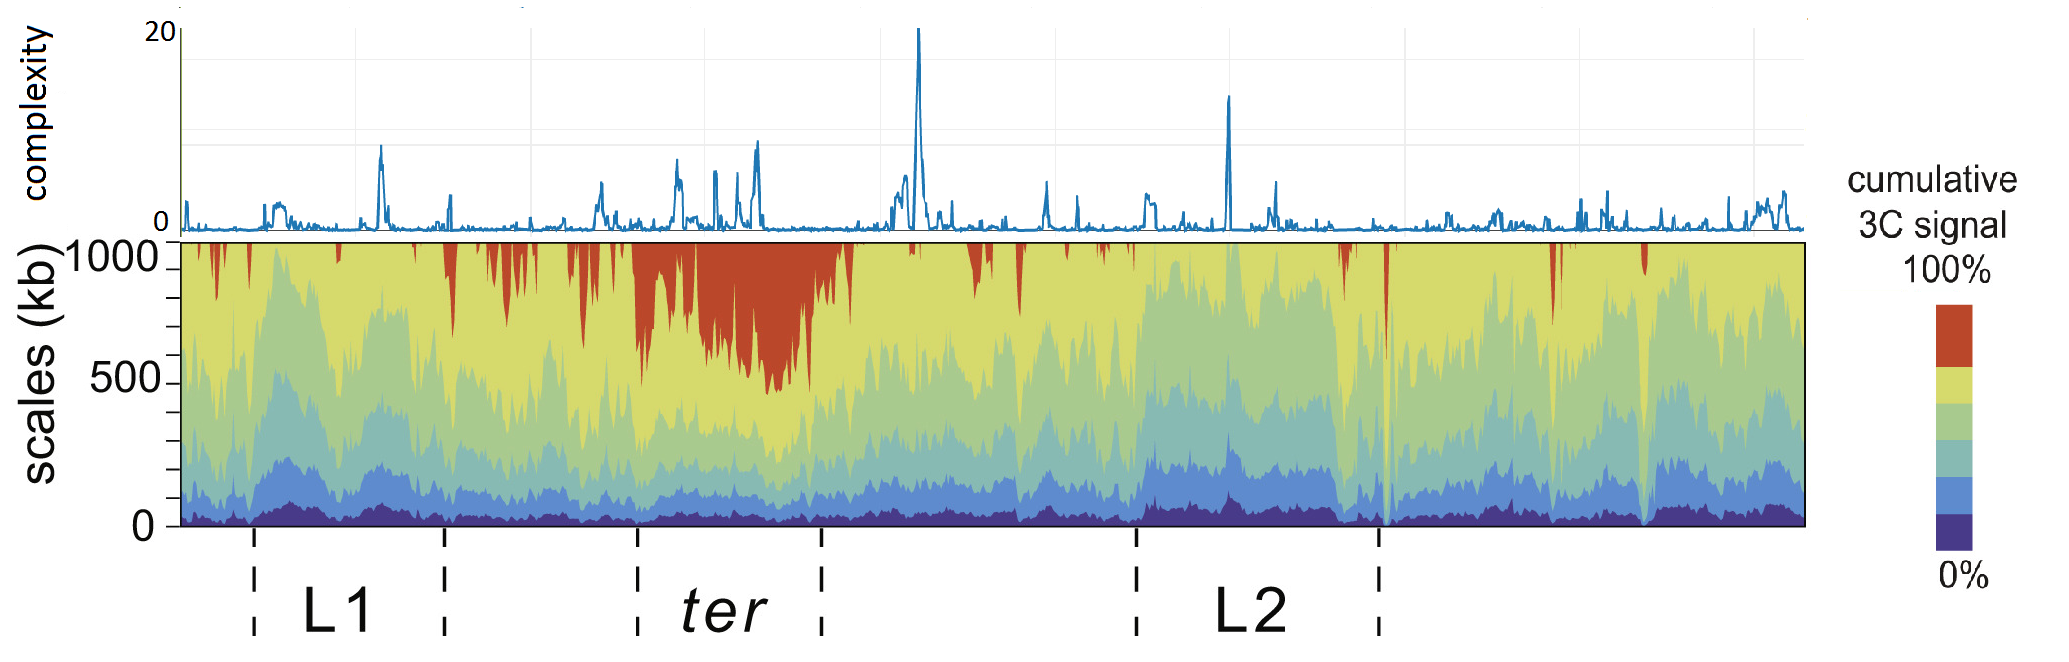
\includegraphics [width=0.9\textwidth] {Dissertation/images/complex_hic/hic_scalogram_complexity_coli.png}
    \caption{Сравнение профиля вариабельности с шкаллограммой хромосомных контактов из публикации \cite{lioy2018multiscale}.}
    \label{img:scalogram_complexity_coli}
\end{figure}

 Для оценки статистической значимости связи мы использовали линейные модели, связывающие плотность контактов в фиксированном диапазоне длин и значение вариабельности. Плотность контактов $S$ для гена с индексом $i$ считалась как сумма значений нормированной матрицы контактов $M$: $S_i = \sum_{j=1}^J M[i,i+j] $. Далее, мы строили линейные модели для связи $V_i \sim S_i$, где $V$ - это уровень изменчивости. Нами была выявлена статистически значимая зависимость между уровнем изменчивости генома и суммой межхромосомных контактов, как для бактерий \textit{E. coli}, так и \textit{B. subtilis}. 
 
 На рисунке~\ref{img:hic_coli_subtilis} приведено значение p-value для линейных моделей, связывающих значение между уровнем вариабельности генома (рассчитанным с размером окна в 20 генов) и суммой контактов, рассчитанных в окнах различного размера. В случае  \textit{E. coli} наибольшее соответствие достигается при размере окна суммирования равному 15 тысяч п.о., а в случае \textit{B. subtilis} --- 10 тысяч п.о.. Это различие согласуется с различием в средней длине генов: для \textit{B. subtilis} она равна 867 нуклеотидам, а для \textit{E. coli} --- 929 нуклеотидам.

\begin{figure}[!ht] 
  \center
  \subcaptionbox{}{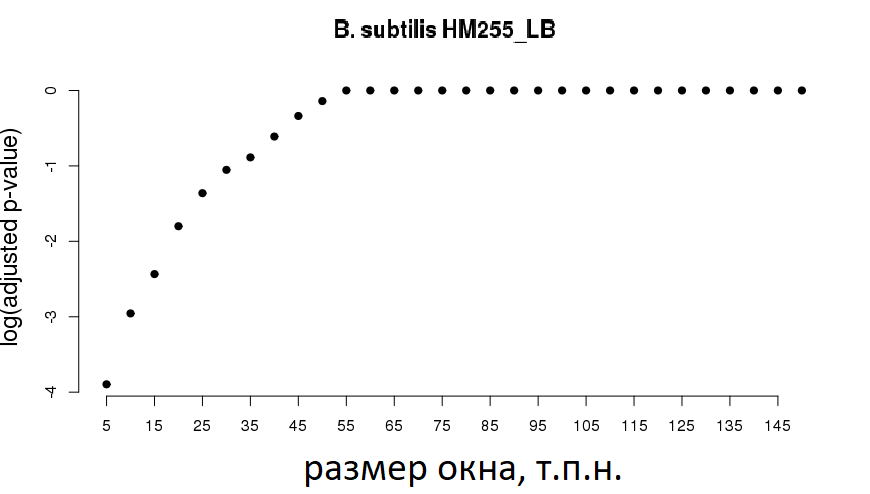
\includegraphics[width=0.6\textwidth]{Dissertation/images/complex_hic/bac_lb.png}}\hfill
  \subcaptionbox{}{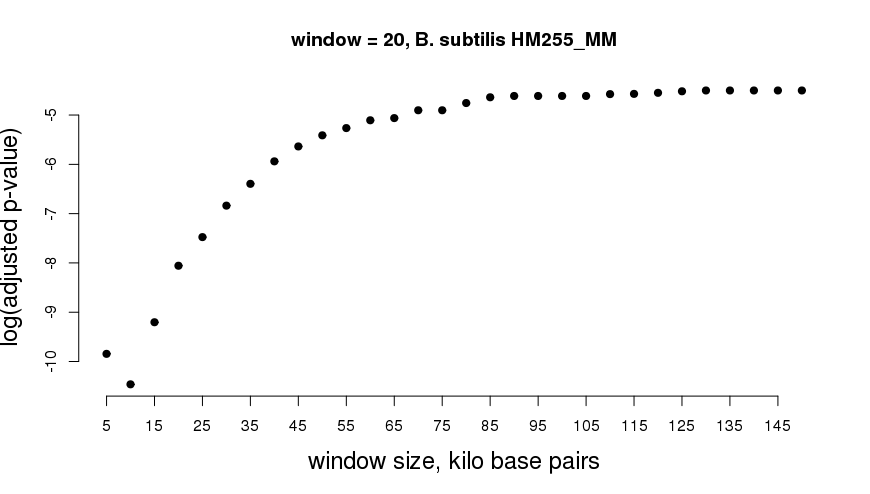
\includegraphics[width=0.6\textwidth]{Dissertation/images/complex_hic/bac_mm.png}}\hfill
  \subcaptionbox{}{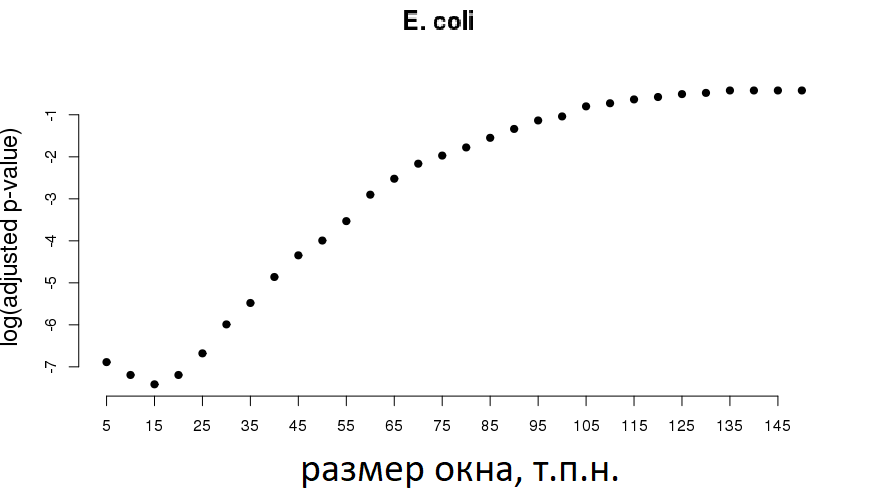
\includegraphics[width=0.6\textwidth]{Dissertation/images/complex_hic/ecoli_20.png}}

  \caption{Зависимость уровня статистической значимости (значение $p-value$) связи между уровнем изменчивости генома и плотностью хромосомных контактов. Размер окна (в тысячах пар нуклеотидов), по которому производилось суммирование значений нормированной матрицы хромосомных контактов, отложен по оси абсцисс. Десятичный логарифм значения p-value линейной модели отложен на оси ординат. На А и Б приведены значения для \textit{B. subtilis} в условиях роста на богатой среде и бедной среде, соответственно; на В приведены значения для \textit{E. coli}.} 
  \label{img:hic_coli_subtilis}  
\end{figure}

Статистическая значимость сохраняется также и при удалении главной и второстепенной диагоналей в матрице контактов (рекомендации сотрудников MIT, \url{https://www.biostars.org/p/208512/}). Так, для \textit{E. coli} значимость связи между вариабельностью и плотностью контактов в пределах 20 тысяч п.о. составляет $p-value = 1.23*10^{-7})$. Значимость ранговой корреляции при этом составила $p-value < 2.2*10^{-16}$. 
Хотя связь между уровнем вариабельности и плотностью хромосомных контактов статистически значима, она объясняет лишь малую долю вариабельности вариабельности. Так, значение $R^2$ для \textit{E. coli} составляет 0.04, а для \textit{B. subtilis} $R^2 = 0.06$.

% script is here /data4/bio/operonTravel_d4/compare_with_3c_ver2/look_with_cumuluted_contacts_v2.r





